% Options for packages loaded elsewhere
\PassOptionsToPackage{unicode}{hyperref}
\PassOptionsToPackage{hyphens}{url}
%
\documentclass[
  oneside]{book}
\title{Introduction to multi-omics data analysis}
\author{University of Turku}
\date{2022-01-08}

\usepackage{amsmath,amssymb}
\usepackage{lmodern}
\usepackage{iftex}
\ifPDFTeX
  \usepackage[T1]{fontenc}
  \usepackage[utf8]{inputenc}
  \usepackage{textcomp} % provide euro and other symbols
\else % if luatex or xetex
  \usepackage{unicode-math}
  \defaultfontfeatures{Scale=MatchLowercase}
  \defaultfontfeatures[\rmfamily]{Ligatures=TeX,Scale=1}
\fi
% Use upquote if available, for straight quotes in verbatim environments
\IfFileExists{upquote.sty}{\usepackage{upquote}}{}
\IfFileExists{microtype.sty}{% use microtype if available
  \usepackage[]{microtype}
  \UseMicrotypeSet[protrusion]{basicmath} % disable protrusion for tt fonts
}{}
\makeatletter
\@ifundefined{KOMAClassName}{% if non-KOMA class
  \IfFileExists{parskip.sty}{%
    \usepackage{parskip}
  }{% else
    \setlength{\parindent}{0pt}
    \setlength{\parskip}{6pt plus 2pt minus 1pt}}
}{% if KOMA class
  \KOMAoptions{parskip=half}}
\makeatother
\usepackage{xcolor}
\IfFileExists{xurl.sty}{\usepackage{xurl}}{} % add URL line breaks if available
\IfFileExists{bookmark.sty}{\usepackage{bookmark}}{\usepackage{hyperref}}
\hypersetup{
  pdftitle={Introduction to multi-omics data analysis},
  pdfauthor={University of Turku},
  hidelinks,
  pdfcreator={LaTeX via pandoc}}
\urlstyle{same} % disable monospaced font for URLs
\usepackage[top=30mm,left=15mm]{geometry}
\usepackage{color}
\usepackage{fancyvrb}
\newcommand{\VerbBar}{|}
\newcommand{\VERB}{\Verb[commandchars=\\\{\}]}
\DefineVerbatimEnvironment{Highlighting}{Verbatim}{commandchars=\\\{\}}
% Add ',fontsize=\small' for more characters per line
\usepackage{framed}
\definecolor{shadecolor}{RGB}{248,248,248}
\newenvironment{Shaded}{\begin{snugshade}}{\end{snugshade}}
\newcommand{\AlertTok}[1]{\textcolor[rgb]{0.94,0.16,0.16}{#1}}
\newcommand{\AnnotationTok}[1]{\textcolor[rgb]{0.56,0.35,0.01}{\textbf{\textit{#1}}}}
\newcommand{\AttributeTok}[1]{\textcolor[rgb]{0.77,0.63,0.00}{#1}}
\newcommand{\BaseNTok}[1]{\textcolor[rgb]{0.00,0.00,0.81}{#1}}
\newcommand{\BuiltInTok}[1]{#1}
\newcommand{\CharTok}[1]{\textcolor[rgb]{0.31,0.60,0.02}{#1}}
\newcommand{\CommentTok}[1]{\textcolor[rgb]{0.56,0.35,0.01}{\textit{#1}}}
\newcommand{\CommentVarTok}[1]{\textcolor[rgb]{0.56,0.35,0.01}{\textbf{\textit{#1}}}}
\newcommand{\ConstantTok}[1]{\textcolor[rgb]{0.00,0.00,0.00}{#1}}
\newcommand{\ControlFlowTok}[1]{\textcolor[rgb]{0.13,0.29,0.53}{\textbf{#1}}}
\newcommand{\DataTypeTok}[1]{\textcolor[rgb]{0.13,0.29,0.53}{#1}}
\newcommand{\DecValTok}[1]{\textcolor[rgb]{0.00,0.00,0.81}{#1}}
\newcommand{\DocumentationTok}[1]{\textcolor[rgb]{0.56,0.35,0.01}{\textbf{\textit{#1}}}}
\newcommand{\ErrorTok}[1]{\textcolor[rgb]{0.64,0.00,0.00}{\textbf{#1}}}
\newcommand{\ExtensionTok}[1]{#1}
\newcommand{\FloatTok}[1]{\textcolor[rgb]{0.00,0.00,0.81}{#1}}
\newcommand{\FunctionTok}[1]{\textcolor[rgb]{0.00,0.00,0.00}{#1}}
\newcommand{\ImportTok}[1]{#1}
\newcommand{\InformationTok}[1]{\textcolor[rgb]{0.56,0.35,0.01}{\textbf{\textit{#1}}}}
\newcommand{\KeywordTok}[1]{\textcolor[rgb]{0.13,0.29,0.53}{\textbf{#1}}}
\newcommand{\NormalTok}[1]{#1}
\newcommand{\OperatorTok}[1]{\textcolor[rgb]{0.81,0.36,0.00}{\textbf{#1}}}
\newcommand{\OtherTok}[1]{\textcolor[rgb]{0.56,0.35,0.01}{#1}}
\newcommand{\PreprocessorTok}[1]{\textcolor[rgb]{0.56,0.35,0.01}{\textit{#1}}}
\newcommand{\RegionMarkerTok}[1]{#1}
\newcommand{\SpecialCharTok}[1]{\textcolor[rgb]{0.00,0.00,0.00}{#1}}
\newcommand{\SpecialStringTok}[1]{\textcolor[rgb]{0.31,0.60,0.02}{#1}}
\newcommand{\StringTok}[1]{\textcolor[rgb]{0.31,0.60,0.02}{#1}}
\newcommand{\VariableTok}[1]{\textcolor[rgb]{0.00,0.00,0.00}{#1}}
\newcommand{\VerbatimStringTok}[1]{\textcolor[rgb]{0.31,0.60,0.02}{#1}}
\newcommand{\WarningTok}[1]{\textcolor[rgb]{0.56,0.35,0.01}{\textbf{\textit{#1}}}}
\usepackage{longtable,booktabs,array}
\usepackage{calc} % for calculating minipage widths
% Correct order of tables after \paragraph or \subparagraph
\usepackage{etoolbox}
\makeatletter
\patchcmd\longtable{\par}{\if@noskipsec\mbox{}\fi\par}{}{}
\makeatother
% Allow footnotes in longtable head/foot
\IfFileExists{footnotehyper.sty}{\usepackage{footnotehyper}}{\usepackage{footnote}}
\makesavenoteenv{longtable}
\usepackage{graphicx}
\makeatletter
\def\maxwidth{\ifdim\Gin@nat@width>\linewidth\linewidth\else\Gin@nat@width\fi}
\def\maxheight{\ifdim\Gin@nat@height>\textheight\textheight\else\Gin@nat@height\fi}
\makeatother
% Scale images if necessary, so that they will not overflow the page
% margins by default, and it is still possible to overwrite the defaults
% using explicit options in \includegraphics[width, height, ...]{}
\setkeys{Gin}{width=\maxwidth,height=\maxheight,keepaspectratio}
% Set default figure placement to htbp
\makeatletter
\def\fps@figure{htbp}
\makeatother
\setlength{\emergencystretch}{3em} % prevent overfull lines
\providecommand{\tightlist}{%
  \setlength{\itemsep}{0pt}\setlength{\parskip}{0pt}}
\setcounter{secnumdepth}{5}
\usepackage{booktabs}
\usepackage{booktabs}
\usepackage{longtable}
\usepackage{array}
\usepackage{multirow}
\usepackage{wrapfig}
\usepackage{float}
\usepackage{colortbl}
\usepackage{pdflscape}
\usepackage{tabu}
\usepackage{threeparttable}
\usepackage{threeparttablex}
\usepackage[normalem]{ulem}
\usepackage{makecell}
\usepackage{xcolor}
\ifLuaTeX
  \usepackage{selnolig}  % disable illegal ligatures
\fi
\usepackage[]{natbib}
\bibliographystyle{apalike}

\begin{document}
\maketitle

{
\setcounter{tocdepth}{1}
\tableofcontents
}
\hypertarget{overview}{%
\chapter{Overview}\label{overview}}

\textbf{Welcome to the multi-omics data analysis workshop}

Figure source: Moreno-Indias \emph{et al}. (2021) \href{https://doi.org/10.3389/fmicb.2021.635781}{Statistical and Machine Learning Techniques in Human Microbiome Studies: Contemporary Challenges and Solutions}. Frontiers in Microbiology 12:11.

\hypertarget{introduction}{%
\section{Introduction}\label{introduction}}

This course is based on \href{https://microbiome.github.io}{\emph{miaverse}} (mia = \textbf{MI}crobiome \textbf{A}nalysis) is an
R/Bioconductor framework for microbiome data science. It extends another popular framework, \href{https://joey711.github.io/phyloseq/}{phyloseq}.

The miaverse consists of an efficient data structure, an
associated package ecosystem, demonstration data sets, and open
documentation. These are explained in more detail in the online book
\href{https://microbiome.github.io/OMA}{Orchestrating Microbiome Analysis}.

This workshop material walks you through example workflows for multi-omics data
analysis covering data access, exploration, analysis, visualization and reproducible
reporting. \textbf{You can run the workflow by simply copy-pasting the
examples.} For advanced material, you can test and modify further
examples from the \href{https://microbiome.github.io/OMA}{OMA book}, or try
to apply the techniques to your own data.

\hypertarget{learning-goals-to-do}{%
\section{Learning goals {[}TO DO{]}}\label{learning-goals-to-do}}

This workshop provides an overview of bioinformatics
tools for multi-omics studies, ranging from data
preprocessing to statistical analysis and reproducible reporting.

\textbf{Target audience} Advanced students and applied researchers who wish
to develop their skills in microbial community analysis. {[}TO DO{]}

\textbf{Venue} {[}TO DO{]}

\hypertarget{acknowledgments}{%
\section{Acknowledgments}\label{acknowledgments}}

\textbf{Citation} ``Introduction to microbiome data science (2021). URL: \url{https://microbiome.github.io}''.

\citet{FindingPheno2022workshop}

We thank Felix Ernst, Sudarshan Shetty, and other \href{https://microbiome.github.io}{miaverse
developers} who have contributed open
resources that supported the development of the training material.

\textbf{Contact} \href{http://datascience.utu.fi}{Leo Lahti}, University of Turku, Finland

\textbf{License} All material is released under the open \href{LICENSE}{CC BY-NC-SA 3.0 License}.

\textbf{Source code}

The source code of this repository is fully reproducible and contains
the Rmd files with executable code. All files can be rendered at one
go by running the file \url{main.R}. You can check the file for
details on how to clone the repository and convert it into a gitbook,
although this is not necessary for the training.

\begin{itemize}
\tightlist
\item
  Landing page (html): \href{https://microbiome.github.io/course_2022_FindingPheno/}{workshop teaching material}
\item
  Source code (github): \href{https://github.com/microbiome/course_2022_FindingPheno}{workshop teaching material}
\end{itemize}

\hypertarget{program}{%
\chapter{Program}\label{program}}

The workshop takes place on the 13th and 14th of January from 11am -- 6pm
(EET). Short breaks will be scheduled between sessions.

The practical sessions consists of a set of example
multi-omics analysis workflows. It is assumed that you
have already installed the required software. Do not hesitate to ask
support from the course assistants.

\hypertarget{day-1}{%
\section{Day 1}\label{day-1}}

\textbf{Lectures}

\begin{itemize}
\item
  Metagenomics - Kata
\item
  Metabolomics - Pande
\item
  Multiomics - Leo
\end{itemize}

\textbf{Practical}

\begin{itemize}
\item
  Data import and exploration
\item
  Beta diversity
\end{itemize}

\begin{center}\rule{0.5\linewidth}{0.5pt}\end{center}

\hypertarget{day-2}{%
\section{Day 2}\label{day-2}}

\textbf{Lectures}

\begin{itemize}
\item
  ML - Matti
\item
  Gergely individual-based modeling
\item
  Data integration - Leo
\end{itemize}

\textbf{Practical ML}

\begin{itemize}
\item
  Unsupervised learning: UMAP clustering
\item
  Supervised learning: Random forest
\item
  Model selection and evaluation
\end{itemize}

\hypertarget{getting-started}{%
\chapter{Getting started}\label{getting-started}}

\hypertarget{checklist-before-the-workshop}{%
\section{Checklist (before the workshop)}\label{checklist-before-the-workshop}}

Install the following software in advance in order to avoid
unnecessary delays and leaving more time for the workshop contents.

\begin{itemize}
\item
  \href{https://www.r-project.org/}{R (version \textgreater4.1.0)}
\item
  \href{https://www.rstudio.com/products/rstudio/download/}{RStudio};
  choose ``Rstudio Desktop'' to download the latest version. Optional
  but preferred. For further details, check the \href{https://www.rstudio.com/}{Rstudio home
  page}.
\item
  Install and load the required R packages
\end{itemize}

\hypertarget{support-and-resources}{%
\section{Support and resources}\label{support-and-resources}}

For online support on installation and other matters, you can join us at:

\begin{itemize}
\tightlist
\item
  Users: \href{https://gitter.im/microbiome/miaverse?utm_source=badge\&utm_medium=badge\&utm_campaign=pr-badge\&utm_content=badge}{miaverse Gitter channel}
\item
  Developers: \href{https://bioc-community.herokuapp.com}{Bioconductor Slack} \#microbiomeexperiment channel (ask for an invitation)
\end{itemize}

\hypertarget{installing-and-loading-the-required-r-packages}{%
\section{Installing and loading the required R packages}\label{installing-and-loading-the-required-r-packages}}

This section shows how to install and load all required packages into
the R session. Only uninstalled packages are installed.

\begin{Shaded}
\begin{Highlighting}[]
\CommentTok{\# List of packages that we need from cran and bioc }
\NormalTok{cran\_pkg }\OtherTok{\textless{}{-}} \FunctionTok{c}\NormalTok{(}\StringTok{"BiocManager"}\NormalTok{, }\StringTok{"bookdown"}\NormalTok{, }\StringTok{"dplyr"}\NormalTok{, }\StringTok{"ecodist"}\NormalTok{, }\StringTok{"ggplot2"}\NormalTok{, }
              \StringTok{"gridExtra"}\NormalTok{, }\StringTok{"kableExtra"}\NormalTok{, }\StringTok{"knitr"}\NormalTok{, }\StringTok{"scales"}\NormalTok{, }\StringTok{"vegan"}\NormalTok{, }\StringTok{"caret"}\NormalTok{,}
              \StringTok{"ranger"}\NormalTok{, }\StringTok{"stringr"}\NormalTok{, }\StringTok{"pheatmap"}\NormalTok{)}
\NormalTok{bioc\_pkg }\OtherTok{\textless{}{-}} \FunctionTok{c}\NormalTok{(}\StringTok{"ANCOMBC"}\NormalTok{, }\StringTok{"ape"}\NormalTok{, }\StringTok{"DESeq2"}\NormalTok{,  }\StringTok{"DirichletMultinomial"}\NormalTok{, }\StringTok{"mia"}\NormalTok{,}
              \StringTok{"miaViz"}\NormalTok{, }\StringTok{"microbiomeDataSets"}\NormalTok{)}

\CommentTok{\# Gets those packages that are already installed}
\NormalTok{cran\_pkg\_already\_installed }\OtherTok{\textless{}{-}}\NormalTok{ cran\_pkg[ cran\_pkg }\SpecialCharTok{\%in\%} \FunctionTok{installed.packages}\NormalTok{() ]}
\NormalTok{bioc\_pkg\_already\_installed }\OtherTok{\textless{}{-}}\NormalTok{ bioc\_pkg[ bioc\_pkg }\SpecialCharTok{\%in\%} \FunctionTok{installed.packages}\NormalTok{() ]}

\CommentTok{\# Gets those packages that need to be installed}
\NormalTok{cran\_pkg\_to\_be\_installed }\OtherTok{\textless{}{-}} \FunctionTok{setdiff}\NormalTok{(cran\_pkg, cran\_pkg\_already\_installed)}
\NormalTok{bioc\_pkg\_to\_be\_installed }\OtherTok{\textless{}{-}} \FunctionTok{setdiff}\NormalTok{(bioc\_pkg, bioc\_pkg\_already\_installed)}
\end{Highlighting}
\end{Shaded}

\begin{Shaded}
\begin{Highlighting}[]
\CommentTok{\# If there are packages that need to be installed, installs them from CRAN}
\ControlFlowTok{if}\NormalTok{( }\FunctionTok{length}\NormalTok{(cran\_pkg\_to\_be\_installed) ) \{}
   \FunctionTok{install.packages}\NormalTok{(cran\_pkg\_to\_be\_installed)}
\NormalTok{\}}
\end{Highlighting}
\end{Shaded}

\begin{Shaded}
\begin{Highlighting}[]
\CommentTok{\# If there are packages that need to be installed, installs them from Bioconductor}
\ControlFlowTok{if}\NormalTok{( }\FunctionTok{length}\NormalTok{(bioc\_pkg\_to\_be\_installed) ) \{}
\NormalTok{   BiocManager}\SpecialCharTok{::}\FunctionTok{install}\NormalTok{(bioc\_pkg\_to\_be\_installed, }\AttributeTok{ask =}\NormalTok{ F)}
\NormalTok{\}}
\end{Highlighting}
\end{Shaded}

Now all required packages are installed, so let's load them into the session.
Some function names occur in multiple packages. That is why miaverse's packages
mia and miaViz are prioritized. Packages that are loaded first have higher priority.

\begin{Shaded}
\begin{Highlighting}[]
\CommentTok{\# Reorders bioc packages, so that mia and miaViz are first}
\NormalTok{bioc\_pkg }\OtherTok{\textless{}{-}} \FunctionTok{c}\NormalTok{(bioc\_pkg[ bioc\_pkg }\SpecialCharTok{\%in\%} \FunctionTok{c}\NormalTok{(}\StringTok{"mia"}\NormalTok{, }\StringTok{"miaViz"}\NormalTok{) ], }
\NormalTok{              bioc\_pkg[ }\SpecialCharTok{!}\NormalTok{bioc\_pkg }\SpecialCharTok{\%in\%} \FunctionTok{c}\NormalTok{(}\StringTok{"mia"}\NormalTok{, }\StringTok{"miaViz"}\NormalTok{) ] ) }

\CommentTok{\# Loading all packages into session. Returns true if package was successfully loaded.}
\NormalTok{loaded }\OtherTok{\textless{}{-}} \FunctionTok{sapply}\NormalTok{(}\FunctionTok{c}\NormalTok{(bioc\_pkg, cran\_pkg), require, }\AttributeTok{character.only =} \ConstantTok{TRUE}\NormalTok{)}
\FunctionTok{as.data.frame}\NormalTok{(loaded)}
\end{Highlighting}
\end{Shaded}

\begin{verbatim}
##                      loaded
## mia                    TRUE
## miaViz                 TRUE
## ANCOMBC                TRUE
## ape                    TRUE
## DESeq2                 TRUE
## DirichletMultinomial   TRUE
## microbiomeDataSets     TRUE
## BiocManager            TRUE
## bookdown               TRUE
## dplyr                  TRUE
## ecodist                TRUE
## ggplot2                TRUE
## gridExtra              TRUE
## kableExtra             TRUE
## knitr                  TRUE
## scales                 TRUE
## vegan                  TRUE
## caret                  TRUE
## ranger                 TRUE
## stringr                TRUE
## pheatmap               TRUE
\end{verbatim}

\hypertarget{data}{%
\chapter{Data}\label{data}}

This section demonstrates how to import data in R.

\hypertarget{data-structure}{%
\section{Data structure}\label{data-structure}}

Such analysis using the miaverse framework, are based upon core data structures
including SingleCellExperiment (SCE), SummarizedExperiment (SE), TreeSummarizedExperiment (TreeSE) and MultiAssayExperiment (MAE) \href{https://microbiome.github.io/course_2022_miaverse/study-material.html\#resources-for-treesummarizedexperiment}{(resources)}.

Multi-assay data can be stored in \href{https://microbiome.github.io/OMA/containers.html\#alternative-experiments}{altExp}
slot of TreeSE or \href{https://microbiome.github.io/OMA/containers.html\#multiassayexperiments}{MAE} data container.

Different data sets are first imported into SE or TreeSE data container similarly to the case when only one data set is present. After that different data sets are combined into the same data container. Result is one TreeSE object with alternative experiment in altExp slot, or MAE object with multiple experiment in its experiment slot.

\hypertarget{example-data}{%
\section{Example data}\label{example-data}}

As an example data, we use data from following publication: Hintikka L et al.~(2021) \href{https://www.mdpi.com/1660-4601/18/8/4049}{Xylo-oligosaccharides in prevention of hepatic steatosis and adipose tissue inflammation: associating taxonomic and metabolomic patterns in fecal microbiotas with biclustering}.

This example data can be loaded from \href{https://bioconductor.org/packages/release/data/experiment/html/microbiomeDataSets.html}{microbiomeDataSets}. The data is already in MAE format. It includes three different experiments: microbial abundance data, metabolite concentrations, and data about different biomarkers.

\hypertarget{importing-data-in-r}{%
\section{Importing data in R}\label{importing-data-in-r}}

\begin{Shaded}
\begin{Highlighting}[]
\FunctionTok{library}\NormalTok{(stringr)}

\CommentTok{\# Load the data}
\NormalTok{mae }\OtherTok{\textless{}{-}}\NormalTok{ microbiomeDataSets}\SpecialCharTok{::}\FunctionTok{HintikkaXOData}\NormalTok{()}

\CommentTok{\# Drop off those bacteria that do not include information in Phylum or lower levels}
\NormalTok{mae[[}\DecValTok{1}\NormalTok{]] }\OtherTok{\textless{}{-}}\NormalTok{ mae[[}\DecValTok{1}\NormalTok{]][}\SpecialCharTok{!}\FunctionTok{is.na}\NormalTok{(}\FunctionTok{rowData}\NormalTok{(mae[[}\DecValTok{1}\NormalTok{]])}\SpecialCharTok{$}\NormalTok{Phylum), ]}

\CommentTok{\# Clean taxonomy data, so that names do not include addtional characters}
\FunctionTok{rowData}\NormalTok{(mae[[}\DecValTok{1}\NormalTok{]]) }\OtherTok{\textless{}{-}} \FunctionTok{DataFrame}\NormalTok{(}\FunctionTok{apply}\NormalTok{(}\FunctionTok{rowData}\NormalTok{(mae[[}\DecValTok{1}\NormalTok{]]), }\DecValTok{2}\NormalTok{, }
\NormalTok{                                     str\_remove, }\AttributeTok{pattern =} \StringTok{".\_[0{-}9]\_\_"}\NormalTok{))}

\NormalTok{mae}
\end{Highlighting}
\end{Shaded}

\begin{verbatim}
## A MultiAssayExperiment object of 3 listed
##  experiments with user-defined names and respective classes.
##  Containing an ExperimentList class object of length 3:
##  [1] microbiota: SummarizedExperiment with 12613 rows and 40 columns
##  [2] metabolites: SummarizedExperiment with 38 rows and 40 columns
##  [3] biomarkers: SummarizedExperiment with 39 rows and 40 columns
## Functionality:
##  experiments() - obtain the ExperimentList instance
##  colData() - the primary/phenotype DataFrame
##  sampleMap() - the sample coordination DataFrame
##  `$`, `[`, `[[` - extract colData columns, subset, or experiment
##  *Format() - convert into a long or wide DataFrame
##  assays() - convert ExperimentList to a SimpleList of matrices
##  exportClass() - save data to flat files
\end{verbatim}

\hypertarget{microbiome-data-exploration}{%
\chapter{Microbiome data exploration}\label{microbiome-data-exploration}}

Now we have loaded the data set into R. Next, let us walk through some
basic operations for data exploration to confirm that the data has all
the necessary components.

\hypertarget{data-structure-1}{%
\section{Data structure}\label{data-structure-1}}

Let us now investigate how taxonomic profiling data is organized in R.

Dimensionality tells us how many taxa and samples the data
contains. As we can see, there are 12613 taxa and 40
samples.

\begin{Shaded}
\begin{Highlighting}[]
\CommentTok{\# mae[[1]]: indexing/retrieving the taxonomic data experiment}
\FunctionTok{dim}\NormalTok{(mae[[}\DecValTok{1}\NormalTok{]])}
\end{Highlighting}
\end{Shaded}

\begin{verbatim}
## [1] 12613    40
\end{verbatim}

The \texttt{rowData} slot contains a taxonomic table. This includes taxonomic
information for each of the 12613 entries. With the \texttt{head()}
command, we can print just the beginning of the table.

The \texttt{rowData} seems to contain information from 7
different taxonomy classes.

\begin{Shaded}
\begin{Highlighting}[]
\NormalTok{knitr}\SpecialCharTok{::}\FunctionTok{kable}\NormalTok{(}\FunctionTok{head}\NormalTok{(}\FunctionTok{rowData}\NormalTok{(mae[[}\DecValTok{1}\NormalTok{]]))) }\SpecialCharTok{\%\textgreater{}\%} 
\NormalTok{  kableExtra}\SpecialCharTok{::}\FunctionTok{kable\_styling}\NormalTok{(}\StringTok{"striped"}\NormalTok{, }
                            \AttributeTok{latex\_options=}\StringTok{"scale\_down"}\NormalTok{) }\SpecialCharTok{\%\textgreater{}\%} 
\NormalTok{  kableExtra}\SpecialCharTok{::}\FunctionTok{scroll\_box}\NormalTok{(}\AttributeTok{width =} \StringTok{"100\%"}\NormalTok{)}
\end{Highlighting}
\end{Shaded}

\begin{table}
\centering
\resizebox{\linewidth}{!}{
\begin{tabular}{l|l|l|l|l|l|l|l}
\hline
  & Phylum & Class & Order & Family & Genus & Species & OTU\\
\hline
GAYR01026362.62.2014 & Proteobacteria & Alphaproteobacteria & Rickettsiales & Mitochondria & Solanum melongena (eggplant) & Solanum melongena (eggplant) & GAYR01026362.62.2014\\
\hline
CVJT01000011.50.2173 & Firmicutes & Bacilli & Bacillales & Staphylococcaceae & Staphylococcus & Staphylococcus aureus & CVJT01000011.50.2173\\
\hline
KF625183.1.1786 & Proteobacteria & Gammaproteobacteria & Enterobacteriales & Enterobacteriaceae & Klebsiella & Klebsiella oxytoca & KF625183.1.1786\\
\hline
AYSG01000002.292.2076 & Firmicutes & Bacilli & Lactobacillales & Streptococcaceae & Streptococcus & Streptococcus thermophilus TH1435 & AYSG01000002.292.2076\\
\hline
CCPS01000022.154.1916 & Proteobacteria & Gammaproteobacteria & Enterobacteriales & Enterobacteriaceae & Escherichia-Shigella & Escherichia coli & CCPS01000022.154.1916\\
\hline
KJ923794.1.1762 & Firmicutes & Bacilli & Bacillales & Staphylococcaceae & Staphylococcus & Staphylococcus aureus & KJ923794.1.1762\\
\hline
\end{tabular}}
\end{table}

The colData slot contains sample metadata. It contains information for all 40 samples.
However, here only the 6 first samples are shown as we use the \texttt{head()} command. There
are 6 columns, that contain information, e.g., about patients' status, and cohort.

\begin{Shaded}
\begin{Highlighting}[]
\CommentTok{\# For simplicity, classify all high{-}fat diets as high{-}fat, and all the low{-}fat }
\CommentTok{\# diets as low{-}fat diets}
\FunctionTok{colData}\NormalTok{(mae)}\SpecialCharTok{$}\NormalTok{Diet }\OtherTok{\textless{}{-}} \FunctionTok{ifelse}\NormalTok{(}\FunctionTok{colData}\NormalTok{(mae)}\SpecialCharTok{$}\NormalTok{Diet }\SpecialCharTok{==} \StringTok{"High{-}fat"} \SpecialCharTok{|} 
                              \FunctionTok{colData}\NormalTok{(mae)}\SpecialCharTok{$}\NormalTok{Diet }\SpecialCharTok{==} \StringTok{"High{-}fat + XOS"}\NormalTok{, }
                            \StringTok{"High{-}fat"}\NormalTok{, }\StringTok{"Low{-}fat"}\NormalTok{)}

\NormalTok{knitr}\SpecialCharTok{::}\FunctionTok{kable}\NormalTok{(}\FunctionTok{head}\NormalTok{(}\FunctionTok{colData}\NormalTok{(mae))) }\SpecialCharTok{\%\textgreater{}\%} 
\NormalTok{  kableExtra}\SpecialCharTok{::}\FunctionTok{kable\_styling}\NormalTok{(}\StringTok{"striped"}\NormalTok{, }
                            \AttributeTok{latex\_options=}\StringTok{"scale\_down"}\NormalTok{) }\SpecialCharTok{\%\textgreater{}\%} 
\NormalTok{  kableExtra}\SpecialCharTok{::}\FunctionTok{scroll\_box}\NormalTok{(}\AttributeTok{width =} \StringTok{"100\%"}\NormalTok{)}
\end{Highlighting}
\end{Shaded}

\begin{table}
\centering
\resizebox{\linewidth}{!}{
\begin{tabular}{l|l|l|l|l|l|r}
\hline
  & Sample & Rat & Site & Diet & Fat & XOS\\
\hline
C1 & C1 & 1 & Cecum & High-fat & High & 0\\
\hline
C2 & C2 & 2 & Cecum & High-fat & High & 0\\
\hline
C3 & C3 & 3 & Cecum & High-fat & High & 0\\
\hline
C4 & C4 & 4 & Cecum & High-fat & High & 0\\
\hline
C5 & C5 & 5 & Cecum & High-fat & High & 0\\
\hline
C6 & C6 & 6 & Cecum & High-fat & High & 0\\
\hline
\end{tabular}}
\end{table}

From here, we can draw summaries of the sample (column) data, for
instance to see what is the diet distribution.

The command \texttt{colData(mae)\$Diet} fetches the data from the
column, and \texttt{table()} creates a table that shows how many times each
class is present, and \texttt{sort()} sorts the table to ascending order.

There are 20
samples from mice having High-fat,
and 20 Low-fat.

\begin{Shaded}
\begin{Highlighting}[]
\FunctionTok{sort}\NormalTok{(}\FunctionTok{table}\NormalTok{(}\FunctionTok{colData}\NormalTok{(mae)}\SpecialCharTok{$}\NormalTok{Diet))}
\end{Highlighting}
\end{Shaded}

\begin{verbatim}
## 
## High-fat  Low-fat 
##       20       20
\end{verbatim}

\hypertarget{transformations}{%
\subsection{Transformations}\label{transformations}}

Microbial abundances are typically `compositional' (relative) in the
current microbiome profiling data sets. This is due to technical
aspects of the data generation process (see e.g.~\href{https://www.frontiersin.org/articles/10.3389/fmicb.2017.02224/full}{Gloor et al.,
2017}).

The next example calculates relative abundances as these are usually easier to
interpret than plain counts. For some statistical models we need to
transform the data into other formats as explained in above link (and
as we will see later).

\begin{Shaded}
\begin{Highlighting}[]
\CommentTok{\# Calculates relative abundances, and stores the table to assays}
\NormalTok{mae[[}\DecValTok{1}\NormalTok{]] }\OtherTok{\textless{}{-}} \FunctionTok{transformCounts}\NormalTok{(mae[[}\DecValTok{1}\NormalTok{]], }\AttributeTok{method =} \StringTok{"relabundance"}\NormalTok{)}
\end{Highlighting}
\end{Shaded}

A variety of standard transformations for microbiome data are available through \href{https://microbiome.github.io/mia/reference/transformCounts.html}{mia R package}.

\hypertarget{aggregation}{%
\subsection{Aggregation}\label{aggregation}}

Microbial species can be called at multiple taxonomic resolutions. We
can easily agglomerate the data based on taxonomic ranks. Here, we
agglomerate the data at Phylum level.

\begin{Shaded}
\begin{Highlighting}[]
\NormalTok{se\_phylum }\OtherTok{\textless{}{-}} \FunctionTok{agglomerateByRank}\NormalTok{(mae[[}\DecValTok{1}\NormalTok{]], }\AttributeTok{rank =} \StringTok{"Phylum"}\NormalTok{)}

\CommentTok{\# Show dimensionality}
\FunctionTok{dim}\NormalTok{(se\_phylum)}
\end{Highlighting}
\end{Shaded}

\begin{verbatim}
## [1] 13 40
\end{verbatim}

Now there are 13 taxa and 40
samples, meaning that there are 13 different
Phylum level taxonomic groups. Looking at the \texttt{rowData} after
agglomeration shows all Firmicutes are combined together, and all
lower rank information is lost.

From the assay we can see that all abundances of taxa that belong to
Firmicutes are summed up.

\begin{Shaded}
\begin{Highlighting}[]
\NormalTok{knitr}\SpecialCharTok{::}\FunctionTok{kable}\NormalTok{(}\FunctionTok{head}\NormalTok{(}\FunctionTok{rowData}\NormalTok{(se\_phylum))) }\SpecialCharTok{\%\textgreater{}\%} 
\NormalTok{  kableExtra}\SpecialCharTok{::}\FunctionTok{kable\_styling}\NormalTok{(}\StringTok{"striped"}\NormalTok{, }
                            \AttributeTok{latex\_options=}\StringTok{"scale\_down"}\NormalTok{) }\SpecialCharTok{\%\textgreater{}\%} 
\NormalTok{  kableExtra}\SpecialCharTok{::}\FunctionTok{scroll\_box}\NormalTok{(}\AttributeTok{width =} \StringTok{"100\%"}\NormalTok{)}
\end{Highlighting}
\end{Shaded}

\begin{table}
\centering
\resizebox{\linewidth}{!}{
\begin{tabular}{l|l|l|l|l|l|l|l}
\hline
  & Phylum & Class & Order & Family & Genus & Species & OTU\\
\hline
Proteobacteria & Proteobacteria & NA & NA & NA & NA & NA & GAYR01026362.62.2014\\
\hline
Firmicutes & Firmicutes & NA & NA & NA & NA & NA & CVJT01000011.50.2173\\
\hline
Cyanobacteria & Cyanobacteria & NA & NA & NA & NA & NA & GEMN01027092.33.1623\\
\hline
Tenericutes & Tenericutes & NA & NA & NA & NA & NA & AM277369.1.1548\\
\hline
Deferribacteres & Deferribacteres & NA & NA & NA & NA & NA & AYGZ01000001.327.1863\\
\hline
Actinobacteria & Actinobacteria & NA & NA & NA & NA & NA & JGZF01000005.1.1534\\
\hline
\end{tabular}}
\end{table}

If you are sharp, you have by now noticed that all the aggregated
values in the above example are NA's (missing data). This is because
the agglomeration is missing abundances for certain taxa, and in that
case the sum is not defined by default (\texttt{na.rm\ =\ FALSE}). We can
ignore the missing values in summing up the data by setting \texttt{na.rm\ =\ TRUE}; then the taxa that do not have information in specified level
will be removed. Those taxa that do not have information in specified
level are agglomerated at lowest possible level that is left after
agglomeration.

\begin{Shaded}
\begin{Highlighting}[]
\NormalTok{temp }\OtherTok{\textless{}{-}} \FunctionTok{rowData}\NormalTok{(}\FunctionTok{agglomerateByRank}\NormalTok{(mae[[}\DecValTok{1}\NormalTok{]], }\AttributeTok{rank =} \StringTok{"Genus"}\NormalTok{))}

\CommentTok{\# Prints those taxa that do not have information at the Genus level (NA)}
\NormalTok{knitr}\SpecialCharTok{::}\FunctionTok{kable}\NormalTok{(}\FunctionTok{head}\NormalTok{(temp[}\FunctionTok{which}\NormalTok{(}\FunctionTok{is.na}\NormalTok{(temp}\SpecialCharTok{$}\NormalTok{Genus)),])) }\SpecialCharTok{\%\textgreater{}\%} 
\NormalTok{  kableExtra}\SpecialCharTok{::}\FunctionTok{kable\_styling}\NormalTok{(}\StringTok{"striped"}\NormalTok{, }
                            \AttributeTok{latex\_options=}\StringTok{"scale\_down"}\NormalTok{) }\SpecialCharTok{\%\textgreater{}\%} 
\NormalTok{  kableExtra}\SpecialCharTok{::}\FunctionTok{scroll\_box}\NormalTok{(}\AttributeTok{width =} \StringTok{"100\%"}\NormalTok{)}
\end{Highlighting}
\end{Shaded}

\begin{table}
\centering
\resizebox{\linewidth}{!}{
\begin{tabular}{l|l|l|l|l|l|l|l}
\hline
  & Phylum & Class & Order & Family & Genus & Species & OTU\\
\hline
Family:uncultured & Proteobacteria & Alphaproteobacteria & Rhodospirillales & uncultured & NA & NA & JRJTB:01000:00983\\
\hline
Family:Ruminococcaceae & Firmicutes & Clostridia & Clostridiales & Ruminococcaceae & NA & NA & JRJTB:00751:00256\\
\hline
Order:Clostridiales & Firmicutes & Clostridia & Clostridiales & NA & NA & NA & JRJTB:03059:01977\\
\hline
Family:Lachnospiraceae & Firmicutes & Clostridia & Clostridiales & Lachnospiraceae & NA & NA & JRJTB:00738:02832\\
\hline
Family:Peptostreptococcaceae & Firmicutes & Clostridia & Clostridiales & Peptostreptococcaceae & NA & NA & JRJTB:01731:00274\\
\hline
Family:Pasteurellaceae & Proteobacteria & Gammaproteobacteria & Pasteurellales & Pasteurellaceae & NA & NA & JRJTB:01960:01703\\
\hline
\end{tabular}}
\end{table}

Here agglomeration is done similarly, but na.rm = TRUE

\begin{Shaded}
\begin{Highlighting}[]
\NormalTok{temp2 }\OtherTok{\textless{}{-}} \FunctionTok{rowData}\NormalTok{(}\FunctionTok{agglomerateByRank}\NormalTok{(mae[[}\DecValTok{1}\NormalTok{]], }\AttributeTok{rank =} \StringTok{"Genus"}\NormalTok{, }\AttributeTok{na.rm =} \ConstantTok{TRUE}\NormalTok{))}

\FunctionTok{print}\NormalTok{(}\FunctionTok{paste0}\NormalTok{(}\StringTok{"Agglomeration with na.rm = FALSE: "}\NormalTok{, }\FunctionTok{dim}\NormalTok{(temp)[}\DecValTok{1}\NormalTok{], }\StringTok{" taxa."}\NormalTok{))}
\end{Highlighting}
\end{Shaded}

\begin{verbatim}
## [1] "Agglomeration with na.rm = FALSE: 277 taxa."
\end{verbatim}

\begin{Shaded}
\begin{Highlighting}[]
\FunctionTok{print}\NormalTok{(}\FunctionTok{paste0}\NormalTok{(}\StringTok{"Agglomeration with na.rm = TRUE: "}\NormalTok{, }\FunctionTok{dim}\NormalTok{(temp2)[}\DecValTok{1}\NormalTok{], }\StringTok{" taxa."}\NormalTok{))}
\end{Highlighting}
\end{Shaded}

\begin{verbatim}
## [1] "Agglomeration with na.rm = TRUE: 262 taxa."
\end{verbatim}

The \href{https://microbiome.github.io/mia/reference/index.html}{mia
package}
contains further examples on various data agglomeration and splitting
options.

\hypertarget{visualization}{%
\section{Visualization}\label{visualization}}

The \href{https://microbiome.github.io/miaViz/}{miaViz package} facilitates
data visualization. Let us plot the Phylum level abundances.

\begin{Shaded}
\begin{Highlighting}[]
\CommentTok{\# Here we specify "relabundance" to be abundance table that we use for plotting.}
\CommentTok{\# Note that we can use agglomerated or non{-}agglomerated mae[[1]] as an input, because}
\CommentTok{\# the function agglomeration is built{-}in option. }

\CommentTok{\# Legend does not fit into picture, so its height is reduced.}
\NormalTok{plot\_abundance }\OtherTok{\textless{}{-}} \FunctionTok{plotAbundance}\NormalTok{(mae[[}\DecValTok{1}\NormalTok{]], }\AttributeTok{abund\_values=}\StringTok{"relabundance"}\NormalTok{, }\AttributeTok{rank =} \StringTok{"Phylum"}\NormalTok{) }\SpecialCharTok{+}
  \FunctionTok{theme}\NormalTok{(}\AttributeTok{legend.key.height =} \FunctionTok{unit}\NormalTok{(}\FloatTok{0.5}\NormalTok{, }\StringTok{"cm"}\NormalTok{)) }\SpecialCharTok{+}
  \FunctionTok{scale\_y\_continuous}\NormalTok{(}\AttributeTok{label =}\NormalTok{ scales}\SpecialCharTok{::}\NormalTok{percent)}

\NormalTok{plot\_abundance }
\end{Highlighting}
\end{Shaded}

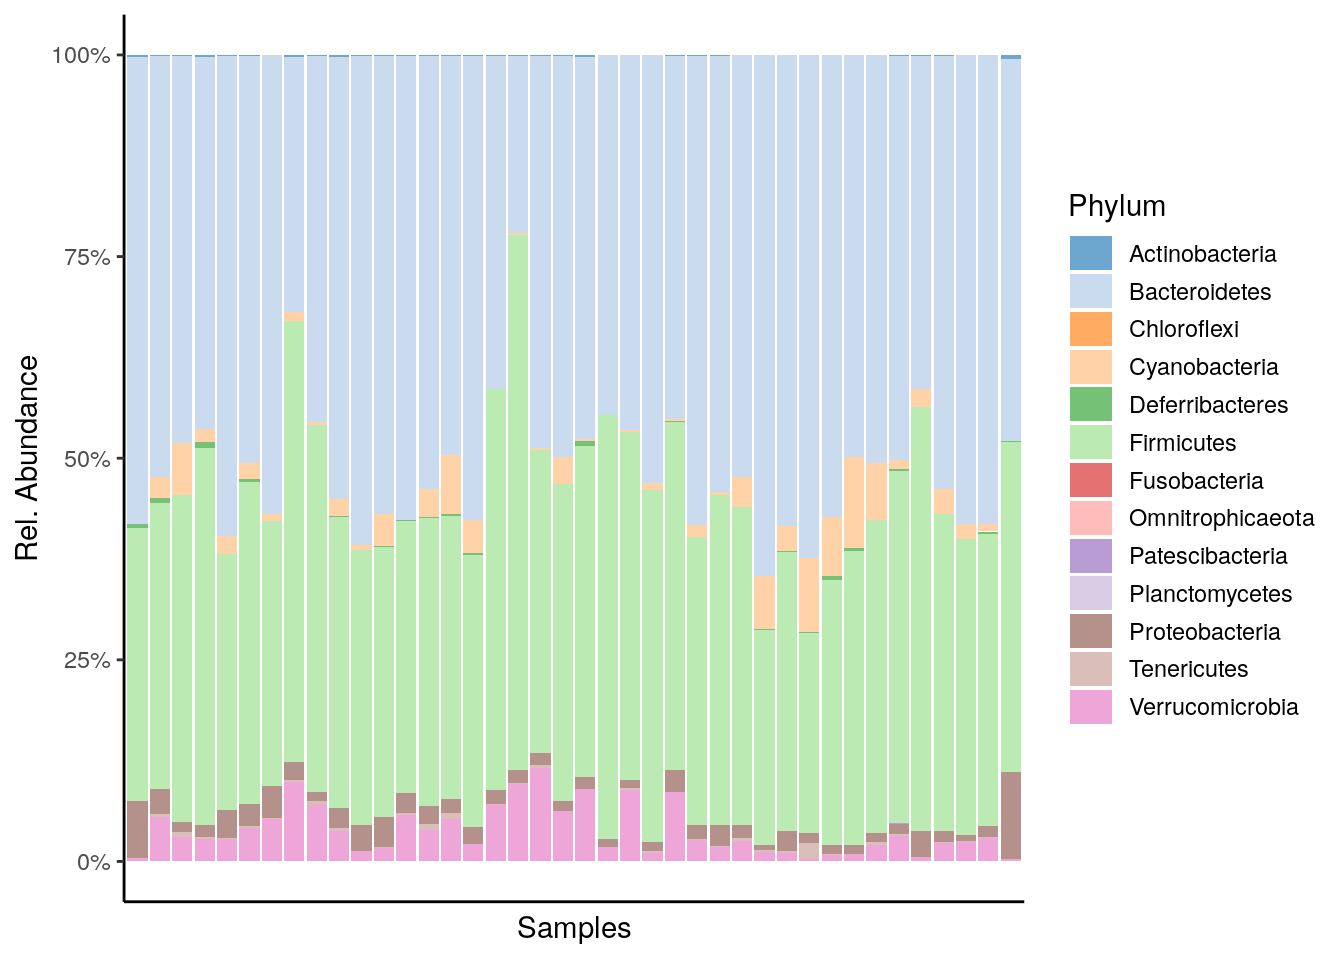
\includegraphics{04-explore_files/figure-latex/unnamed-chunk-10-1.pdf}

\textbf{Density plot} shows the overall abundance distribution for a given
taxonomic group. Let us check the relative abundance of Firmicutes
across the sample collection. The density plot is a smoothened
version of a standard histogram.

The plot shows peak abundances around 30 \%.

\begin{Shaded}
\begin{Highlighting}[]
\CommentTok{\# Subset data by taking only Firmicutes}
\NormalTok{se\_firmicutes }\OtherTok{\textless{}{-}}\NormalTok{ se\_phylum[}\StringTok{"Firmicutes"}\NormalTok{]}

\CommentTok{\# Gets the abundance table}
\NormalTok{abundance\_firmicutes }\OtherTok{\textless{}{-}} \FunctionTok{assay}\NormalTok{(se\_firmicutes, }\StringTok{"relabundance"}\NormalTok{)}

\CommentTok{\# Creates a data frame object, where first column includes abundances}
\NormalTok{firmicutes\_abund\_df }\OtherTok{\textless{}{-}} \FunctionTok{as.data.frame}\NormalTok{(}\FunctionTok{t}\NormalTok{(abundance\_firmicutes))}
\CommentTok{\# Rename the first and only column}
\FunctionTok{colnames}\NormalTok{(firmicutes\_abund\_df) }\OtherTok{\textless{}{-}} \StringTok{"abund"}

\CommentTok{\# Creates a plot. Parameters inside feom\_density are optional. With }
\CommentTok{\# geom\_density(bw=1000), it is possible to adjust bandwidth.}
\NormalTok{firmicutes\_abund\_plot }\OtherTok{\textless{}{-}} \FunctionTok{ggplot}\NormalTok{(firmicutes\_abund\_df, }\FunctionTok{aes}\NormalTok{(}\AttributeTok{x =}\NormalTok{ abund)) }\SpecialCharTok{+} 
  \FunctionTok{geom\_density}\NormalTok{(}\AttributeTok{color=}\StringTok{"darkred"}\NormalTok{, }\AttributeTok{fill=}\StringTok{"lightblue"}\NormalTok{) }\SpecialCharTok{+} 
  \FunctionTok{labs}\NormalTok{(}\AttributeTok{x =} \StringTok{"Relative abundance"}\NormalTok{, }\AttributeTok{title =} \StringTok{"Firmicutes"}\NormalTok{) }\SpecialCharTok{+}
  \FunctionTok{theme\_classic}\NormalTok{() }\SpecialCharTok{+} \CommentTok{\# Changes the background}
  \FunctionTok{scale\_x\_continuous}\NormalTok{(}\AttributeTok{label =}\NormalTok{ scales}\SpecialCharTok{::}\NormalTok{percent)}

\NormalTok{firmicutes\_abund\_plot}
\end{Highlighting}
\end{Shaded}

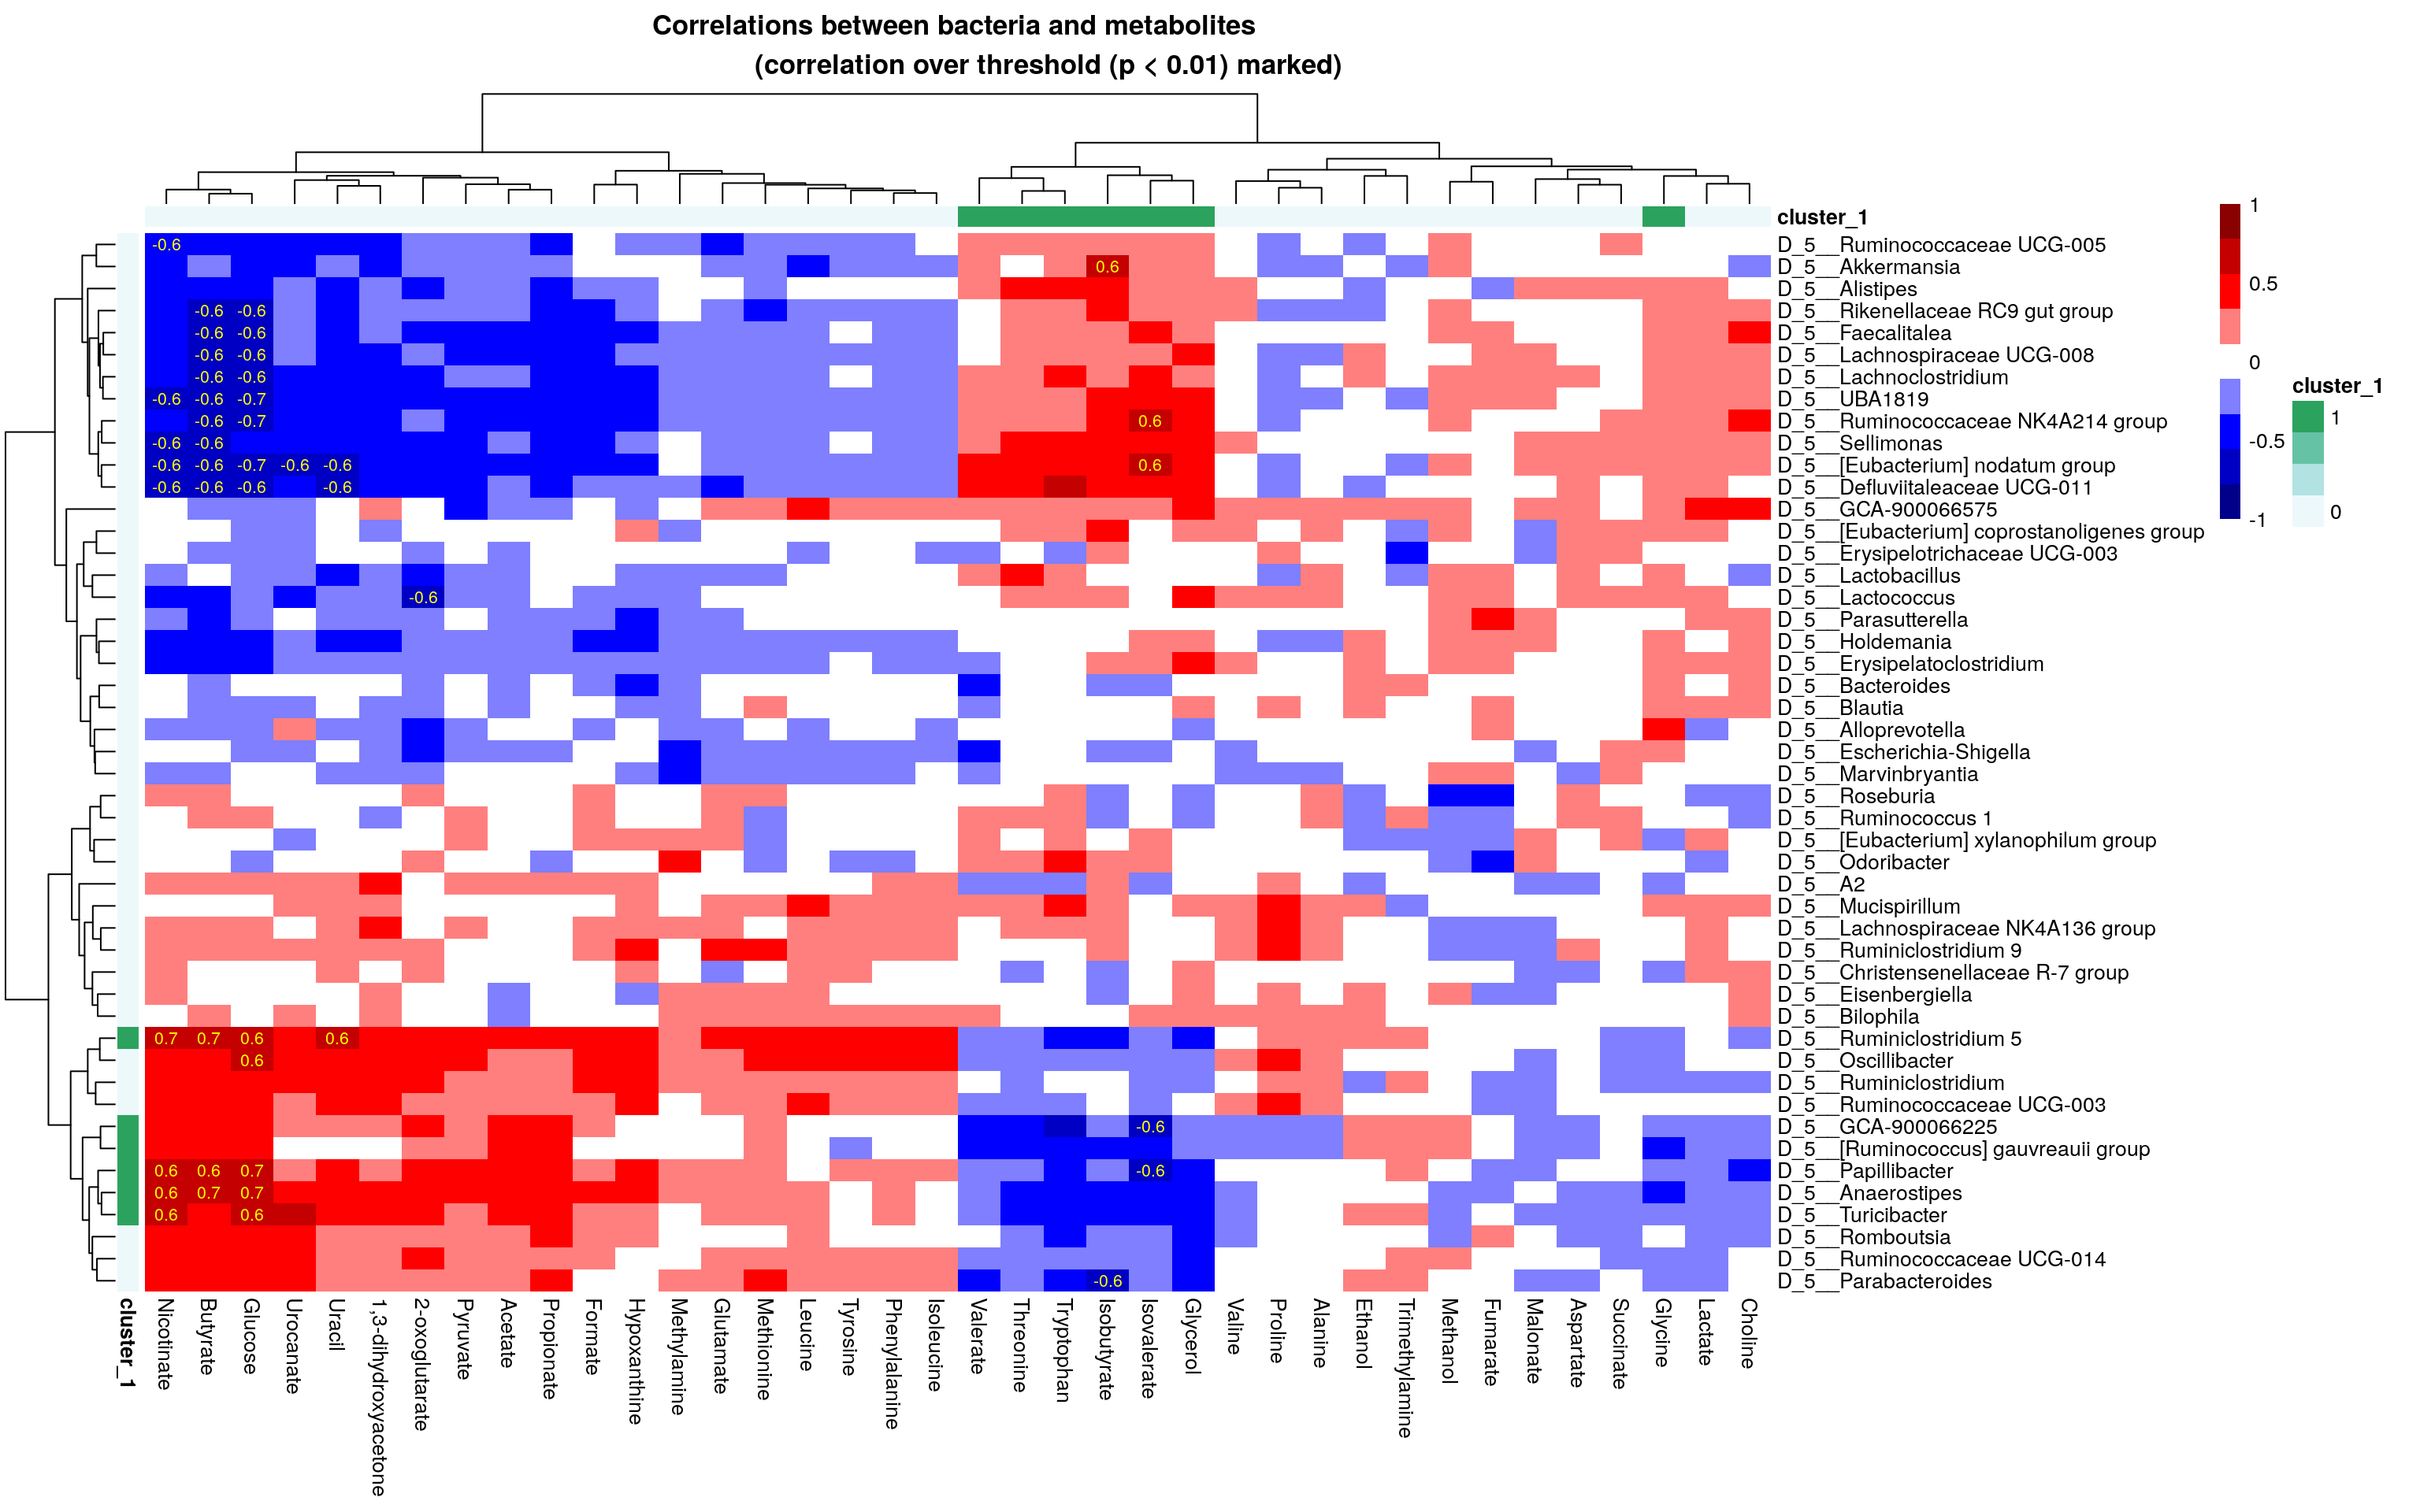
\includegraphics{04-explore_files/figure-latex/unnamed-chunk-11-1.pdf}

For more visualization options and examples, see the \href{https://microbiome.github.io/miaViz/articles/miaViz.html}{miaViz vignette}.

\hypertarget{beta-diversity}{%
\chapter{Beta diversity}\label{beta-diversity}}

Beta diversity is another name for sample dissimilarity. It quantifies
differences in the overall taxonomic composition between two samples.

Common indices include Bray-Curtis, Unifrac, Jaccard index, and the
Aitchison distance. Each of these (dis)similarity measures emphasizes
different aspects. For example, UniFrac incorporates phylogenetic
information, and Jaccard index ignores exact abundances and considers
only presence/absence values. For more background information
and examples, you can check the dedicated section in \href{https://microbiome.github.io/OMA/microbiome-diversity.html\#beta-diversity}{online
book}.

\hypertarget{examples-of-pcoa-with-different-settings}{%
\section{Examples of PCoA with different settings}\label{examples-of-pcoa-with-different-settings}}

Beta diversity estimation generates a (dis)similarity matrix that
contains for each sample (rows) the dissimilarity to any other sample
(columns).

This complex set of pairwise relations can be visualized in
informative ways, and even coupled with other explanatory
variables. As a first step, we compress the information to a lower
dimensionality, or fewer principal components, and then visualize
sample similarity based on that using ordination techniques, such as
Principal Coordinate Analysis (PCoA). PCoA is a non-linear dimension
reduction technique, and with Euclidean distances it is is identical
to the linear PCA (except for potential scaling).

We typically retain just the two (or three) most informative top
components, and ignore the other information. Each sample has a score
on each of these components, and each component measures the variation
across a set of correlated taxa. The top components are then easily
visualized on a two (or three) dimensional display.

Let us next look at some concrete examples.

\hypertarget{pcoa-for-asv-level-data-with-bray-curtis}{%
\subsection{PCoA for ASV-level data with Bray-Curtis}\label{pcoa-for-asv-level-data-with-bray-curtis}}

Let us start with PCoA based on a Bray-Curtis dissimilarity matrix
calculated at Genus level abundances.

\begin{Shaded}
\begin{Highlighting}[]
\CommentTok{\# Pick the relative abundance table}
\NormalTok{rel\_abund\_assay }\OtherTok{\textless{}{-}} \FunctionTok{assays}\NormalTok{(mae[[}\DecValTok{1}\NormalTok{]])}\SpecialCharTok{$}\NormalTok{relabundance}

\CommentTok{\# Calculates Bray{-}Curtis distances between samples. Because taxa is in}
\CommentTok{\# columns, it is used to compare different samples. We transpose the}
\CommentTok{\# assay to get taxa to columns}
\NormalTok{bray\_curtis\_dist }\OtherTok{\textless{}{-}}\NormalTok{ vegan}\SpecialCharTok{::}\FunctionTok{vegdist}\NormalTok{(}\FunctionTok{t}\NormalTok{(rel\_abund\_assay), }\AttributeTok{method =} \StringTok{"bray"}\NormalTok{)}

\CommentTok{\# PCoA}
\NormalTok{bray\_curtis\_pcoa }\OtherTok{\textless{}{-}}\NormalTok{ ecodist}\SpecialCharTok{::}\FunctionTok{pco}\NormalTok{(bray\_curtis\_dist)}

\CommentTok{\# All components could be found here: }
\CommentTok{\# bray\_curtis\_pcoa$vectors}
\CommentTok{\# But we only need the first two to demonstrate what we can do:}
\NormalTok{bray\_curtis\_pcoa\_df }\OtherTok{\textless{}{-}} \FunctionTok{data.frame}\NormalTok{(}\AttributeTok{pcoa1 =}\NormalTok{ bray\_curtis\_pcoa}\SpecialCharTok{$}\NormalTok{vectors[,}\DecValTok{1}\NormalTok{], }
                                  \AttributeTok{pcoa2 =}\NormalTok{ bray\_curtis\_pcoa}\SpecialCharTok{$}\NormalTok{vectors[,}\DecValTok{2}\NormalTok{])}

\CommentTok{\# Create a plot}
\NormalTok{bray\_curtis\_plot }\OtherTok{\textless{}{-}} \FunctionTok{ggplot}\NormalTok{(}\AttributeTok{data =}\NormalTok{ bray\_curtis\_pcoa\_df, }\FunctionTok{aes}\NormalTok{(}\AttributeTok{x=}\NormalTok{pcoa1, }\AttributeTok{y=}\NormalTok{pcoa2)) }\SpecialCharTok{+}
  \FunctionTok{geom\_point}\NormalTok{() }\SpecialCharTok{+}
  \FunctionTok{labs}\NormalTok{(}\AttributeTok{x =} \StringTok{"PC1"}\NormalTok{,}
       \AttributeTok{y =} \StringTok{"PC2"}\NormalTok{, }
       \AttributeTok{title =} \StringTok{"Bray{-}Curtis PCoA"}\NormalTok{) }\SpecialCharTok{+}
  \FunctionTok{theme}\NormalTok{(}\AttributeTok{title =} \FunctionTok{element\_text}\NormalTok{(}\AttributeTok{size =} \DecValTok{10}\NormalTok{)) }\CommentTok{\# makes titles smaller}

\NormalTok{bray\_curtis\_plot}
\end{Highlighting}
\end{Shaded}

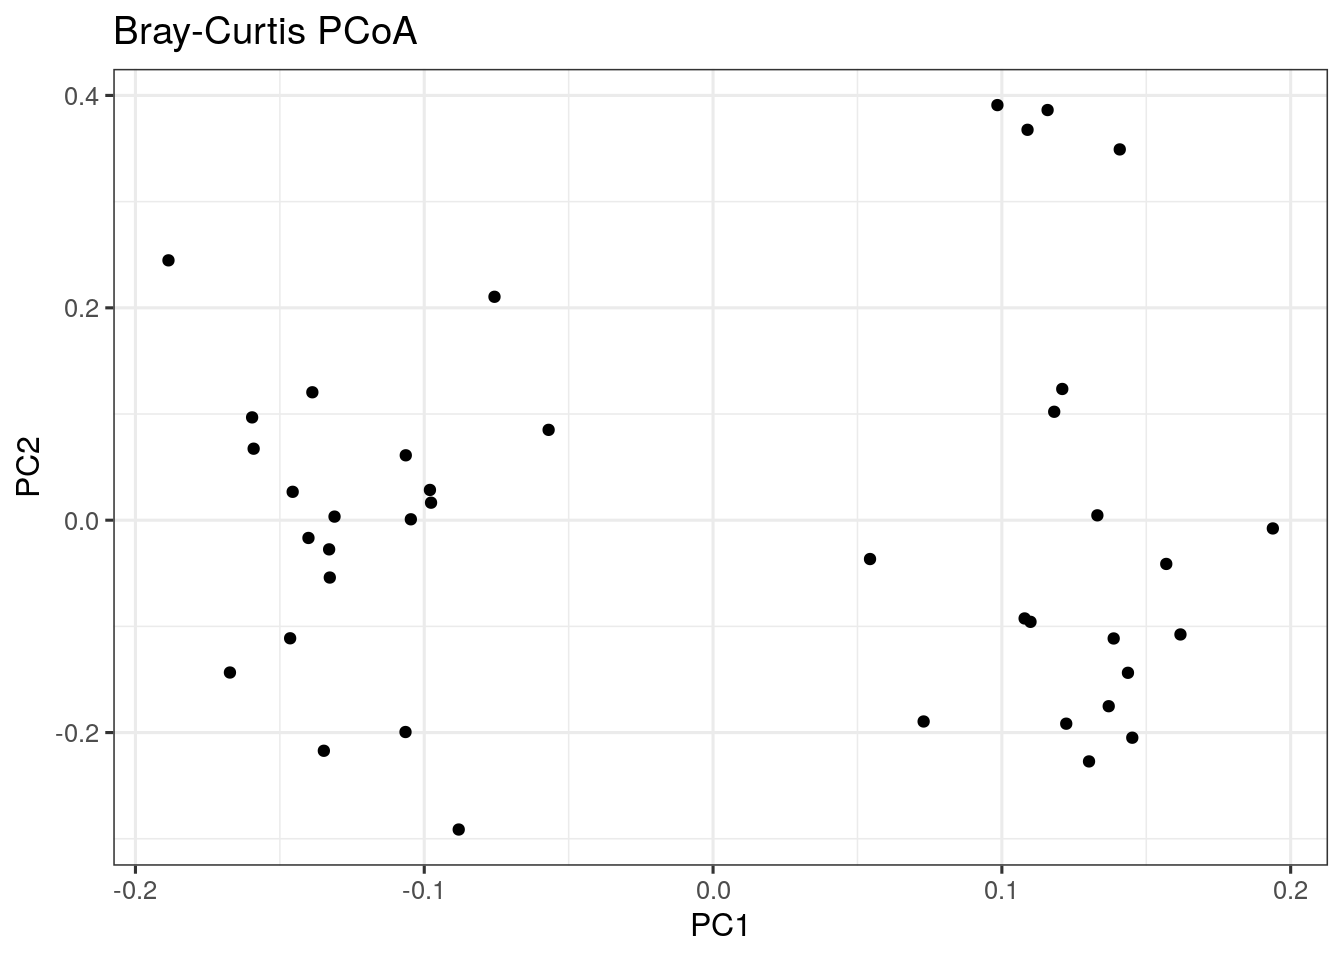
\includegraphics{05-beta_files/figure-latex/pcoa_asv_bc-1.pdf}

\hypertarget{pcoa-for-asv-level-data-with-aitchison-distance}{%
\subsection{PCoA for ASV-level data with Aitchison distance}\label{pcoa-for-asv-level-data-with-aitchison-distance}}

Now the same using Aitchison distance. This metric corresponds to
Euclidean distances between CLR transformed sample abundance vectors.

\begin{Shaded}
\begin{Highlighting}[]
\CommentTok{\# Does clr transformation. Pseudocount is added, because data contains zeros. }
\NormalTok{mae[[}\DecValTok{1}\NormalTok{]] }\OtherTok{\textless{}{-}} \FunctionTok{transformCounts}\NormalTok{(mae[[}\DecValTok{1}\NormalTok{]], }\AttributeTok{method =} \StringTok{"clr"}\NormalTok{, }\AttributeTok{pseudocount =} \DecValTok{1}\NormalTok{)}

\CommentTok{\# Gets clr table}
\NormalTok{clr\_assay }\OtherTok{\textless{}{-}} \FunctionTok{assays}\NormalTok{(mae[[}\DecValTok{1}\NormalTok{]])}\SpecialCharTok{$}\NormalTok{clr}

\CommentTok{\# Transposes it to get taxa to columns}
\NormalTok{clr\_assay }\OtherTok{\textless{}{-}} \FunctionTok{t}\NormalTok{(clr\_assay)}

\CommentTok{\# Calculates Euclidean distances between samples. Because taxa is in columns,}
\CommentTok{\# it is used to compare different samples.}
\NormalTok{euclidean\_dist }\OtherTok{\textless{}{-}}\NormalTok{ vegan}\SpecialCharTok{::}\FunctionTok{vegdist}\NormalTok{(clr\_assay, }\AttributeTok{method =} \StringTok{"euclidean"}\NormalTok{)}

\CommentTok{\# Does principal coordinate analysis}
\NormalTok{euclidean\_pcoa }\OtherTok{\textless{}{-}}\NormalTok{ ecodist}\SpecialCharTok{::}\FunctionTok{pco}\NormalTok{(euclidean\_dist)}

\CommentTok{\# Creates a data frame from principal coordinates}
\NormalTok{euclidean\_pcoa\_df }\OtherTok{\textless{}{-}} \FunctionTok{data.frame}\NormalTok{(}\AttributeTok{pcoa1 =}\NormalTok{ euclidean\_pcoa}\SpecialCharTok{$}\NormalTok{vectors[,}\DecValTok{1}\NormalTok{], }
                                \AttributeTok{pcoa2 =}\NormalTok{ euclidean\_pcoa}\SpecialCharTok{$}\NormalTok{vectors[,}\DecValTok{2}\NormalTok{])}

\CommentTok{\# Creates the plot}
\NormalTok{euclidean\_plot }\OtherTok{\textless{}{-}} \FunctionTok{ggplot}\NormalTok{(}\AttributeTok{data =}\NormalTok{ euclidean\_pcoa\_df, }\FunctionTok{aes}\NormalTok{(}\AttributeTok{x=}\NormalTok{pcoa1, }\AttributeTok{y=}\NormalTok{pcoa2)) }\SpecialCharTok{+}
  \FunctionTok{geom\_point}\NormalTok{() }\SpecialCharTok{+}
  \FunctionTok{labs}\NormalTok{(}\AttributeTok{x =} \StringTok{"PC1"}\NormalTok{,}
       \AttributeTok{y =} \StringTok{"PC2"}\NormalTok{,}
       \AttributeTok{title =} \StringTok{"Euclidean PCoA with CLR transformation"}\NormalTok{) }\SpecialCharTok{+}
  \FunctionTok{theme}\NormalTok{(}\AttributeTok{title =} \FunctionTok{element\_text}\NormalTok{(}\AttributeTok{size =} \DecValTok{12}\NormalTok{)) }\CommentTok{\# makes titles smaller}

\NormalTok{euclidean\_plot}
\end{Highlighting}
\end{Shaded}

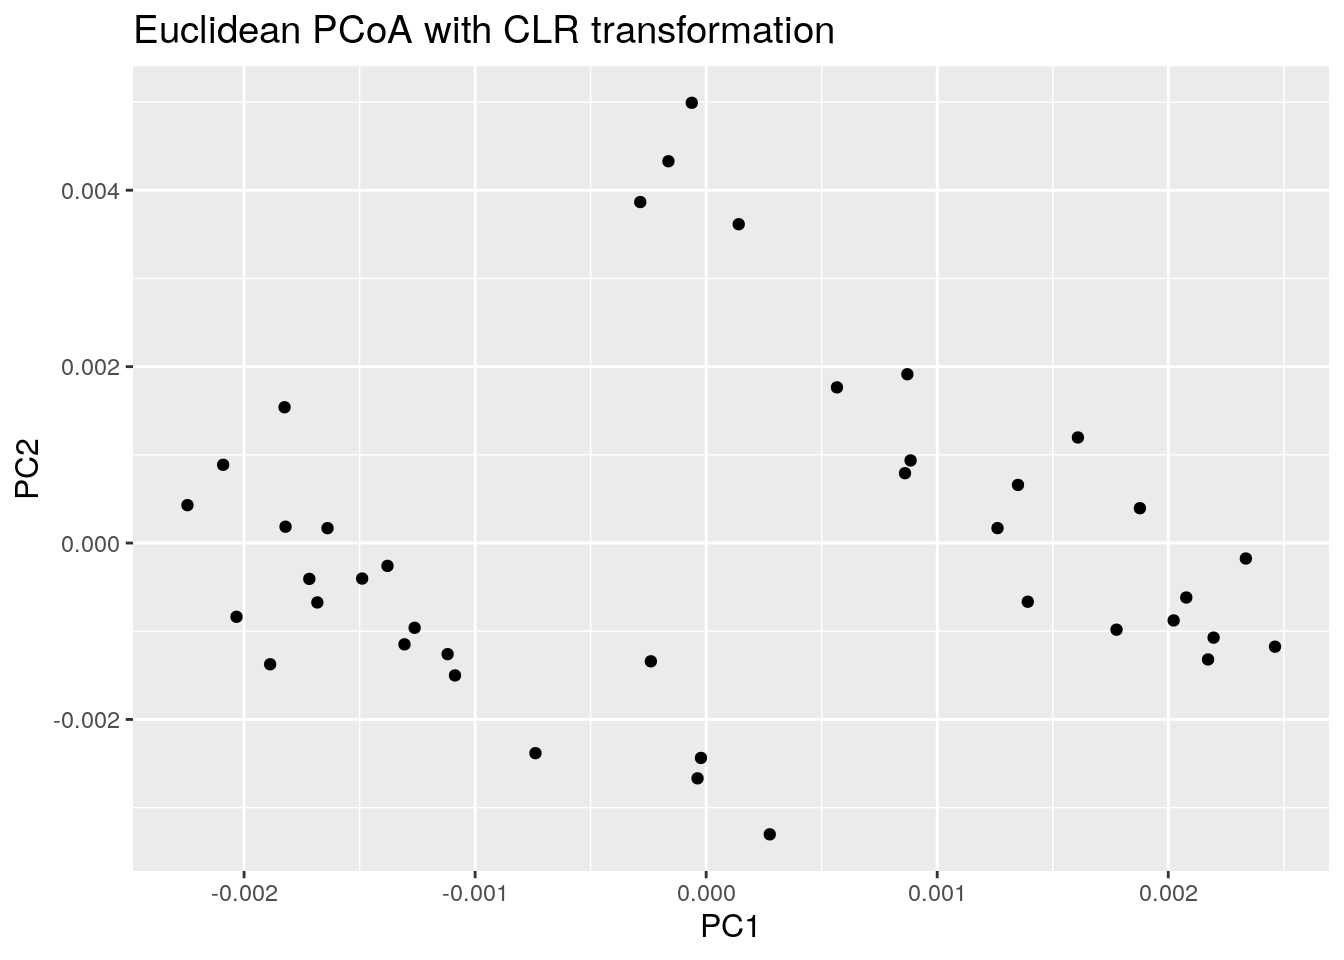
\includegraphics{05-beta_files/figure-latex/pcoa_asv_aitchison-1.pdf}

\hypertarget{pcoa-aggregated-to-phylum-level}{%
\subsection{PCoA aggregated to Phylum level}\label{pcoa-aggregated-to-phylum-level}}

We use again the Aitchison distances in this example but this time applied to the phylum level.

\begin{Shaded}
\begin{Highlighting}[]
\CommentTok{\# Does clr transformation. Psuedocount is added, because data contains zeros. }
\NormalTok{se\_phylum }\OtherTok{\textless{}{-}} \FunctionTok{transformCounts}\NormalTok{(se\_phylum, }\AttributeTok{method =} \StringTok{"clr"}\NormalTok{, }\AttributeTok{pseudocount =} \DecValTok{1}\NormalTok{)}

\CommentTok{\# Gets clr table}
\NormalTok{clr\_phylum\_assay }\OtherTok{\textless{}{-}} \FunctionTok{assays}\NormalTok{(se\_phylum)}\SpecialCharTok{$}\NormalTok{clr}

\CommentTok{\# Transposes it to get taxa to columns}
\NormalTok{clr\_phylum\_assay }\OtherTok{\textless{}{-}} \FunctionTok{t}\NormalTok{(clr\_phylum\_assay)}

\CommentTok{\# Calculates Euclidean distances between samples. Because taxa is in columns,}
\CommentTok{\# it is used to compare different samples.}
\NormalTok{euclidean\_phylum\_dist }\OtherTok{\textless{}{-}}\NormalTok{ vegan}\SpecialCharTok{::}\FunctionTok{vegdist}\NormalTok{(clr\_assay, }\AttributeTok{method =} \StringTok{"euclidean"}\NormalTok{)}

\CommentTok{\# Does principal coordinate analysis}
\NormalTok{euclidean\_phylum\_pcoa }\OtherTok{\textless{}{-}}\NormalTok{ ecodist}\SpecialCharTok{::}\FunctionTok{pco}\NormalTok{(euclidean\_phylum\_dist)}

\CommentTok{\# Creates a data frame from principal coordinates}
\NormalTok{euclidean\_phylum\_pcoa\_df }\OtherTok{\textless{}{-}} \FunctionTok{data.frame}\NormalTok{(}
  \AttributeTok{pcoa1 =}\NormalTok{ euclidean\_phylum\_pcoa}\SpecialCharTok{$}\NormalTok{vectors[,}\DecValTok{1}\NormalTok{], }
  \AttributeTok{pcoa2 =}\NormalTok{ euclidean\_phylum\_pcoa}\SpecialCharTok{$}\NormalTok{vectors[,}\DecValTok{2}\NormalTok{])}

\CommentTok{\# Creates a plot}
\NormalTok{euclidean\_phylum\_plot }\OtherTok{\textless{}{-}} \FunctionTok{ggplot}\NormalTok{(}\AttributeTok{data =}\NormalTok{ euclidean\_phylum\_pcoa\_df,}
  \FunctionTok{aes}\NormalTok{(}\AttributeTok{x=}\NormalTok{pcoa1, }\AttributeTok{y=}\NormalTok{pcoa2)) }\SpecialCharTok{+}
  \FunctionTok{geom\_point}\NormalTok{() }\SpecialCharTok{+}
  \FunctionTok{labs}\NormalTok{(}\AttributeTok{x =} \StringTok{"PC1"}\NormalTok{,}
       \AttributeTok{y =} \StringTok{"PC2"}\NormalTok{,}
       \AttributeTok{title =} \StringTok{"Aitchison distances at Phylum level"}\NormalTok{) }\SpecialCharTok{+}  
  \FunctionTok{theme}\NormalTok{(}\AttributeTok{title =} \FunctionTok{element\_text}\NormalTok{(}\AttributeTok{size =} \DecValTok{12}\NormalTok{)) }\CommentTok{\# makes titles smaller}

\NormalTok{euclidean\_phylum\_plot}
\end{Highlighting}
\end{Shaded}

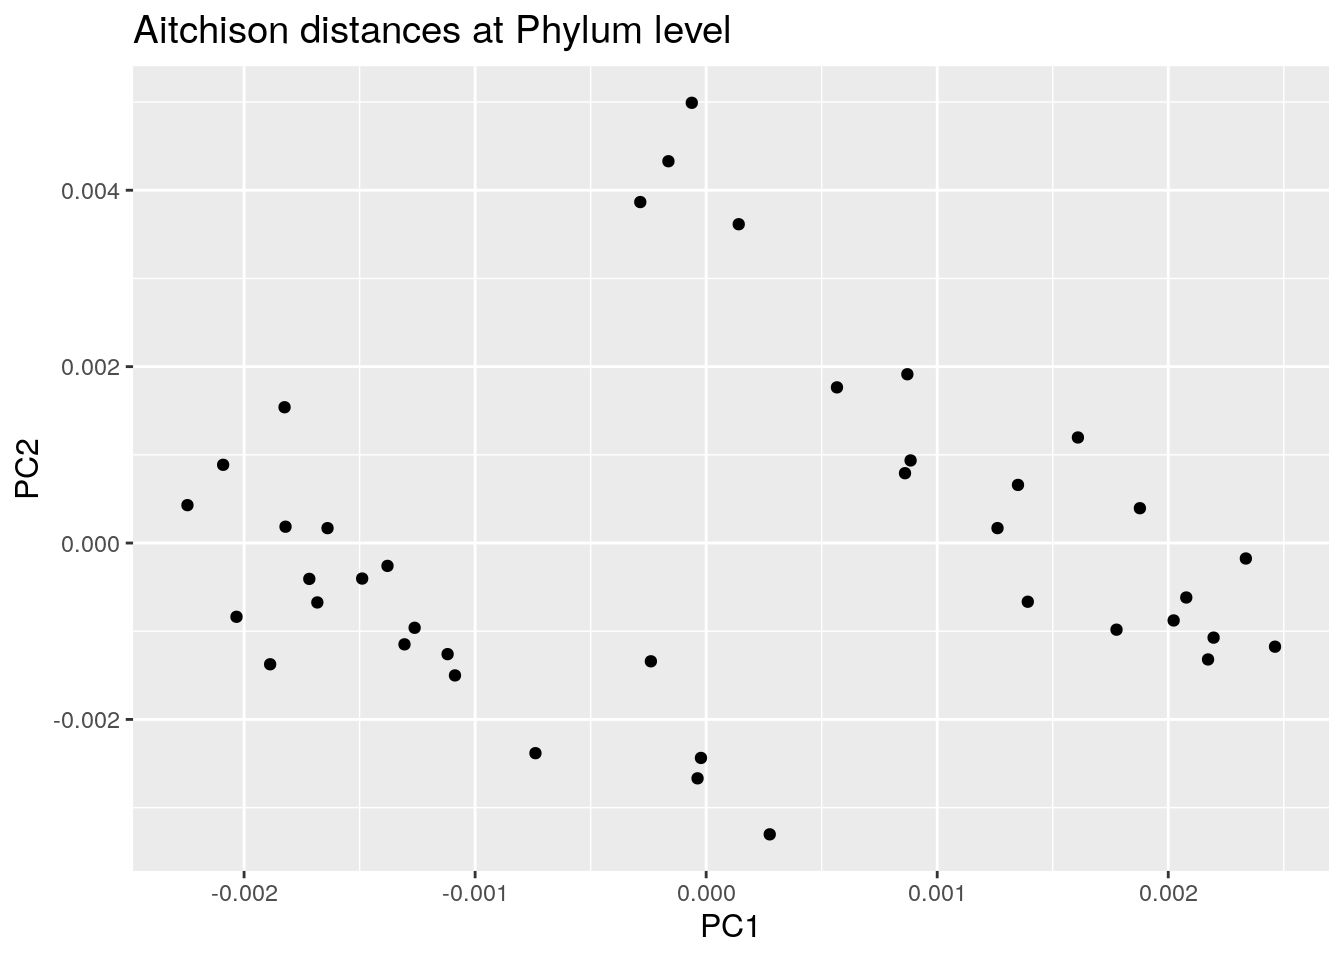
\includegraphics{05-beta_files/figure-latex/pcoa_phylum_aitchison-1.pdf}

\hypertarget{highlighting-external-variables}{%
\section{Highlighting external variables}\label{highlighting-external-variables}}

We can map other variables on the same plot for example by coloring
the points accordingly.

The following is an example with a discrete grouping variable (Diet) shown with colors:

\begin{Shaded}
\begin{Highlighting}[]
\CommentTok{\# Adds the variable we later use for coloring to the data frame}
\NormalTok{euclidean\_diet\_pcoa\_df }\OtherTok{\textless{}{-}} \FunctionTok{cbind}\NormalTok{(euclidean\_pcoa\_df,}
                             \AttributeTok{Diet =} \FunctionTok{colData}\NormalTok{(mae)}\SpecialCharTok{$}\NormalTok{Diet)}

\CommentTok{\# Creates a plot}
\NormalTok{euclidean\_diet\_plot }\OtherTok{\textless{}{-}} \FunctionTok{ggplot}\NormalTok{(}\AttributeTok{data =}\NormalTok{ euclidean\_diet\_pcoa\_df, }
                                        \FunctionTok{aes}\NormalTok{(}\AttributeTok{x=}\NormalTok{pcoa1, }\AttributeTok{y=}\NormalTok{pcoa2,}
                                            \AttributeTok{color =}\NormalTok{ Diet)) }\SpecialCharTok{+}
  \FunctionTok{geom\_point}\NormalTok{() }\SpecialCharTok{+}
  \FunctionTok{labs}\NormalTok{(}\AttributeTok{x =} \StringTok{"PC1"}\NormalTok{,}
       \AttributeTok{y =} \StringTok{"PC2"}\NormalTok{,}
       \AttributeTok{title =} \StringTok{"PCoA with Aitchison distances"}\NormalTok{) }\SpecialCharTok{+}
  \FunctionTok{theme}\NormalTok{(}\AttributeTok{title =} \FunctionTok{element\_text}\NormalTok{(}\AttributeTok{size =} \DecValTok{12}\NormalTok{)) }\CommentTok{\# makes titles smaller}

\NormalTok{euclidean\_diet\_plot}
\end{Highlighting}
\end{Shaded}

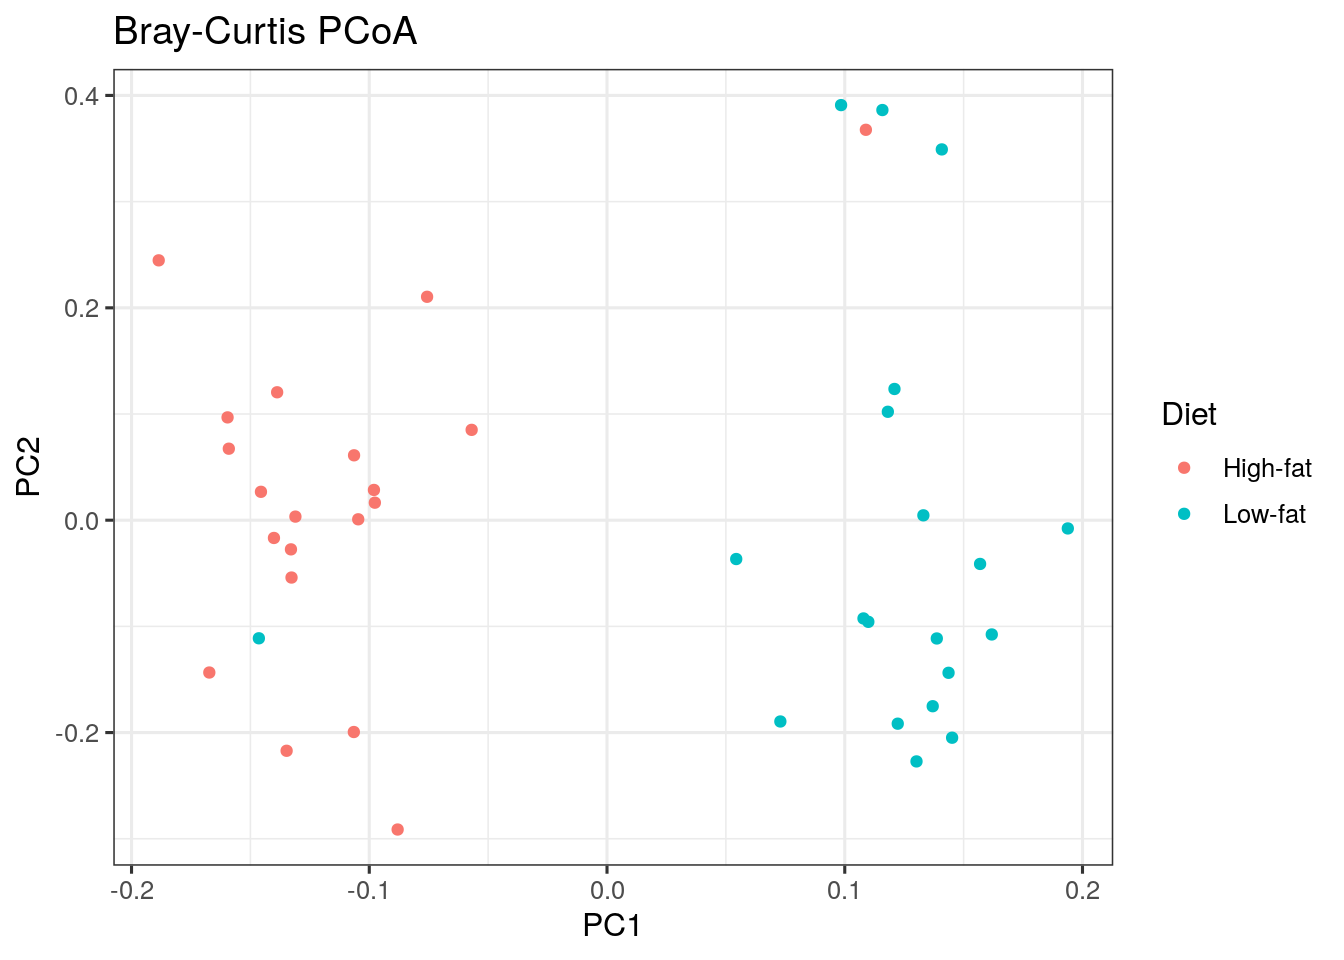
\includegraphics{05-beta_files/figure-latex/pcoa_genus-1.pdf}

PCoA plot in some cases could also be overlayed with a continuous variable. (\href{https://microbiome.github.io/course_2022_miaverse/beta-diversity.html\#pcoa-plot-with-continuous-variable}{see example})

\hypertarget{estimating-associations-with-an-external-variable}{%
\section{Estimating associations with an external variable}\label{estimating-associations-with-an-external-variable}}

Next to visualizing whether any variable is associated with
differences between samples, we can also quantify the strength of the
association between community composition (beta diversity) and
external factors.

The standard way to do this is to perform a so-called permutational
multivariate analysis of variance (PERMANOVA). This method takes as
input the abundance table, which measure of distance you want to base
the test on and a formula that tells the model how you think the
variables are associated with each other.

\begin{Shaded}
\begin{Highlighting}[]
\CommentTok{\# First we get the relative abundance table}
\NormalTok{rel\_abund\_assay }\OtherTok{\textless{}{-}} \FunctionTok{assays}\NormalTok{(mae[[}\DecValTok{1}\NormalTok{]])}\SpecialCharTok{$}\NormalTok{relabundance}

\CommentTok{\# again transpose it to get taxa to columns}
\NormalTok{rel\_abund\_assay }\OtherTok{\textless{}{-}} \FunctionTok{t}\NormalTok{(rel\_abund\_assay)}

\CommentTok{\# then we can perform the method}
\NormalTok{permanova\_diet }\OtherTok{\textless{}{-}}\NormalTok{ vegan}\SpecialCharTok{::}\FunctionTok{adonis}\NormalTok{(rel\_abund\_assay }\SpecialCharTok{\textasciitilde{}}\NormalTok{ Diet,}
                                  \AttributeTok{data =} \FunctionTok{colData}\NormalTok{(mae),}
                                  \AttributeTok{permutations =} \DecValTok{99}\NormalTok{)}

\CommentTok{\# we can obtain a the p value for our predictor:}
\FunctionTok{print}\NormalTok{(}\FunctionTok{paste0}\NormalTok{(}\StringTok{"The test result p{-}value: "}\NormalTok{, }
              \FunctionTok{as.data.frame}\NormalTok{(permanova\_diet}\SpecialCharTok{$}\NormalTok{aov.tab)[}\StringTok{"Diet"}\NormalTok{, }\StringTok{"Pr(\textgreater{}F)"}\NormalTok{]))}
\end{Highlighting}
\end{Shaded}

\begin{verbatim}
## [1] "The test result p-value: 0.01"
\end{verbatim}

The diet variable is significantly associated with
microbiota composition (p-value is less than 0.05).

We can visualize those taxa whose abundances drive the
differences between diets. We first need to extract the model
coefficients of taxa:

\begin{Shaded}
\begin{Highlighting}[]
\CommentTok{\# Gets the coefficients}
\NormalTok{coef }\OtherTok{\textless{}{-}} \FunctionTok{coefficients}\NormalTok{(permanova\_diet)[}\StringTok{"Diet1"}\NormalTok{,]}

\CommentTok{\# Gets the highest coefficients}
\NormalTok{top.coef }\OtherTok{\textless{}{-}} \FunctionTok{sort}\NormalTok{(}\FunctionTok{head}\NormalTok{(coef[}\FunctionTok{rev}\NormalTok{(}\FunctionTok{order}\NormalTok{(}\FunctionTok{abs}\NormalTok{(coef)))],}\DecValTok{20}\NormalTok{))}

\CommentTok{\# Plots the coefficients}
\NormalTok{top\_taxa\_coeffient\_plot }\OtherTok{\textless{}{-}} \FunctionTok{ggplot}\NormalTok{(}\FunctionTok{data.frame}\NormalTok{(}\AttributeTok{x =}\NormalTok{ top.coef,}
                                             \AttributeTok{y =} \FunctionTok{factor}\NormalTok{(}\FunctionTok{names}\NormalTok{(top.coef),}
                         \FunctionTok{unique}\NormalTok{(}\FunctionTok{names}\NormalTok{(top.coef)))),}
                                  \FunctionTok{aes}\NormalTok{(}\AttributeTok{x =}\NormalTok{ x, }\AttributeTok{y =}\NormalTok{ y)) }\SpecialCharTok{+}
  \FunctionTok{geom\_bar}\NormalTok{(}\AttributeTok{stat=}\StringTok{"identity"}\NormalTok{) }\SpecialCharTok{+}
  \FunctionTok{labs}\NormalTok{(}\AttributeTok{x=}\StringTok{""}\NormalTok{, }\AttributeTok{y=}\StringTok{""}\NormalTok{, }\AttributeTok{title=}\StringTok{"Top Taxa"}\NormalTok{) }\SpecialCharTok{+}
  \FunctionTok{theme\_bw}\NormalTok{()}

\NormalTok{top\_taxa\_coeffient\_plot}
\end{Highlighting}
\end{Shaded}

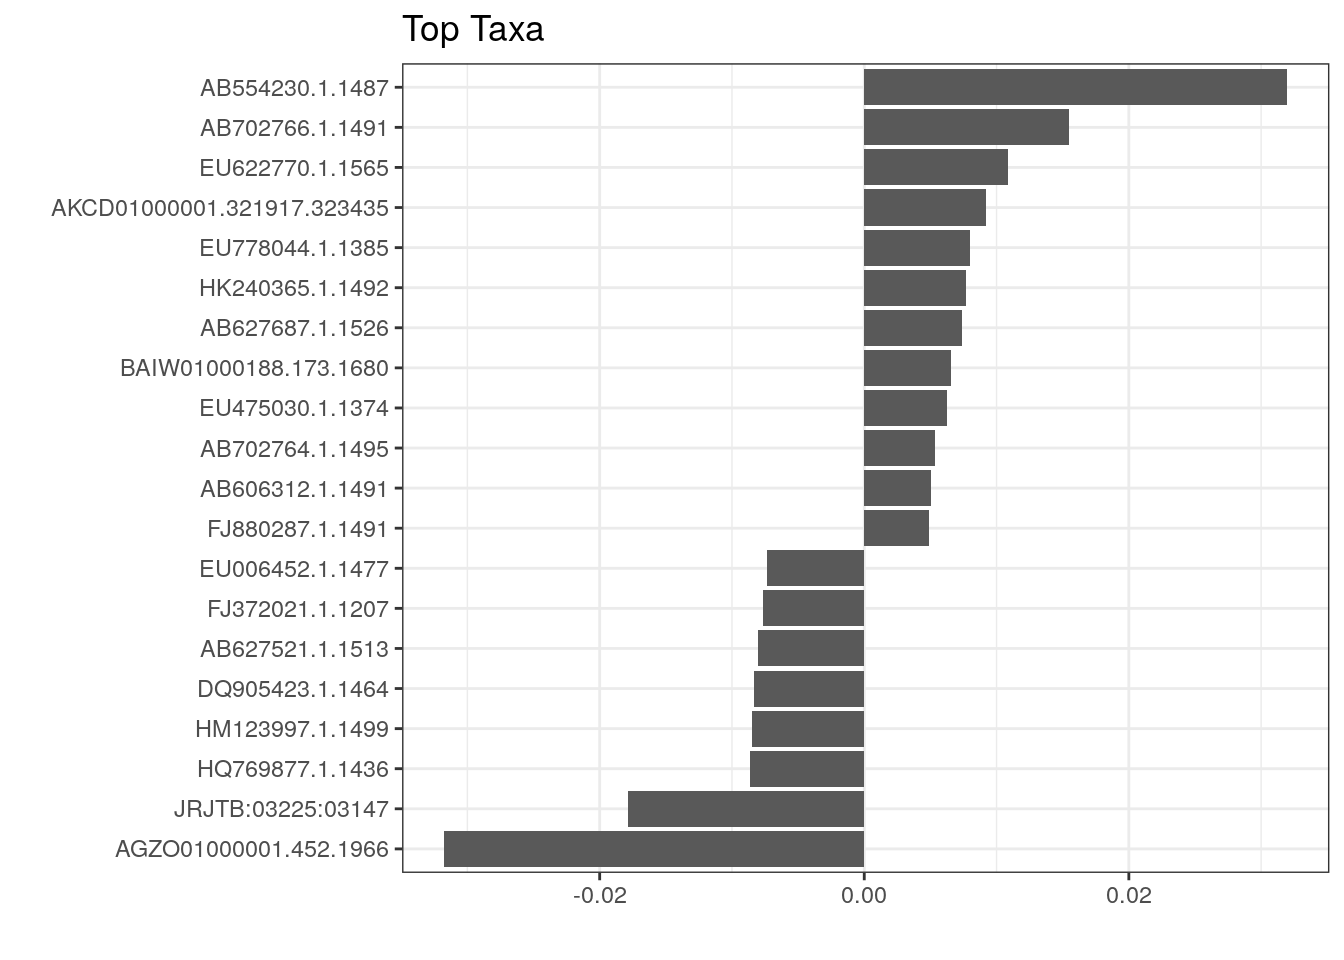
\includegraphics{05-beta_files/figure-latex/permanova_coefs-1.pdf}

The above plot shows taxa as code names, and it is hard to tell which
bacterial groups they represent. However, it is easy to add human readable
names. We can fetch those from our rowData. Here we use Genus level names:

\begin{Shaded}
\begin{Highlighting}[]
\CommentTok{\# Gets corresponding Genus level names and stores them to top.coef}
\NormalTok{names }\OtherTok{\textless{}{-}} \FunctionTok{rowData}\NormalTok{(mae[[}\DecValTok{1}\NormalTok{]])[}\FunctionTok{names}\NormalTok{(top.coef), ][,}\StringTok{"Genus"}\NormalTok{]}

\CommentTok{\# Adds new labels to the plot}
\NormalTok{top\_taxa\_coeffient\_plot }\OtherTok{\textless{}{-}}\NormalTok{ top\_taxa\_coeffient\_plot }\SpecialCharTok{+}
  \FunctionTok{scale\_y\_discrete}\NormalTok{(}\AttributeTok{labels =}\NormalTok{ names) }\CommentTok{\# Adds new labels}
\NormalTok{top\_taxa\_coeffient\_plot}
\end{Highlighting}
\end{Shaded}

\includegraphics{05-beta_files/figure-latex/unnamed-chunk-2-1.pdf}

The same test can be conducted using the oridination from PCoA as follows:

\begin{Shaded}
\begin{Highlighting}[]
\NormalTok{bray\_curtis\_pcoa\_df}\SpecialCharTok{$}\NormalTok{Diet }\OtherTok{\textless{}{-}} \FunctionTok{colData}\NormalTok{(mae)}\SpecialCharTok{$}\NormalTok{Diet}
\NormalTok{p\_values }\OtherTok{\textless{}{-}} \FunctionTok{list}\NormalTok{()}
\ControlFlowTok{for}\NormalTok{(pc }\ControlFlowTok{in} \FunctionTok{c}\NormalTok{(}\StringTok{"pcoa1"}\NormalTok{, }\StringTok{"pcoa2"}\NormalTok{))\{}
  \CommentTok{\# Creates a formula from objects}
\NormalTok{  formula }\OtherTok{\textless{}{-}} \FunctionTok{as.formula}\NormalTok{(}\FunctionTok{paste0}\NormalTok{(pc, }\StringTok{" \textasciitilde{} "}\NormalTok{, }\StringTok{"Diet"}\NormalTok{))}
  \CommentTok{\# Does the permanova analysis}
\NormalTok{  p\_values[[pc]] }\OtherTok{\textless{}{-}}\NormalTok{ vegan}\SpecialCharTok{::}\FunctionTok{adonis}\NormalTok{(formula, }\AttributeTok{data =}\NormalTok{ bray\_curtis\_pcoa\_df,}
                                  \AttributeTok{permutations =} \DecValTok{9999}\NormalTok{, }\AttributeTok{method =} \StringTok{"euclidean"}
\NormalTok{  )}\SpecialCharTok{$}\NormalTok{aov.tab[}\StringTok{"Diet"}\NormalTok{, }\StringTok{"Pr(\textgreater{}F)"}\NormalTok{]}
\NormalTok{\}}

\CommentTok{\# Creates a plot}
\NormalTok{plot }\OtherTok{\textless{}{-}} \FunctionTok{ggplot}\NormalTok{(}\AttributeTok{data =}\NormalTok{ bray\_curtis\_pcoa\_df, }\FunctionTok{aes\_string}\NormalTok{(}\AttributeTok{x =} \StringTok{"pcoa1"}\NormalTok{, }\AttributeTok{y =} \StringTok{"pcoa2"}\NormalTok{, }\AttributeTok{color =} \StringTok{"Diet"}\NormalTok{)) }\SpecialCharTok{+}
  \FunctionTok{geom\_point}\NormalTok{(}\AttributeTok{size =} \DecValTok{3}\NormalTok{) }\SpecialCharTok{+}
  \FunctionTok{labs}\NormalTok{(}\AttributeTok{title =} \FunctionTok{paste0}\NormalTok{(}\StringTok{"PCoA beta diversity ordination for microbiome samples"}\NormalTok{), }\AttributeTok{x =} \FunctionTok{paste0}\NormalTok{(}\StringTok{"PC1 (p = "}\NormalTok{, p\_values[[}\StringTok{"pcoa1"}\NormalTok{]], }\StringTok{")"}\NormalTok{), }\AttributeTok{y =} \FunctionTok{paste0}\NormalTok{(}\StringTok{"PC2 (p = "}\NormalTok{, p\_values[[}\StringTok{"pcoa2"}\NormalTok{]], }\StringTok{")"}\NormalTok{)) }\SpecialCharTok{+}
  \FunctionTok{theme\_bw}\NormalTok{(}\DecValTok{12}\NormalTok{) }

\NormalTok{plot}
\end{Highlighting}
\end{Shaded}

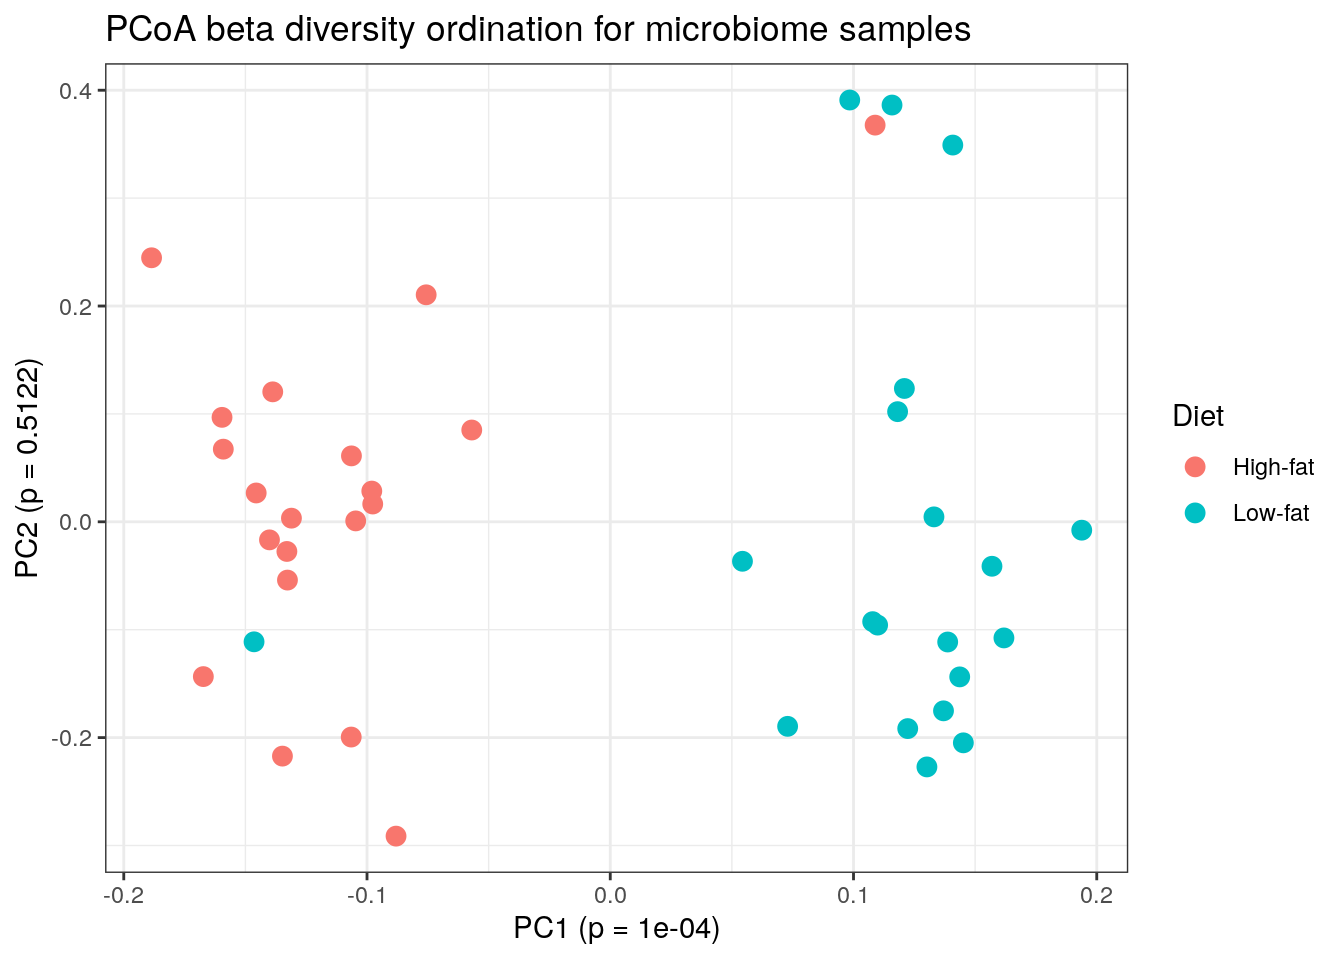
\includegraphics{05-beta_files/figure-latex/unnamed-chunk-3-1.pdf}

There are many alternative and complementary methods for analysing
community composition. For more examples, see a dedicated section on
beta diversity in the \href{https://microbiome.github.io/OMA/microbiome-diversity.html\#beta-diversity}{online
book}.

\hypertarget{community-typing}{%
\section{Community typing}\label{community-typing}}

A dedicated section presenting examples on community typing is in the
\href{https://microbiome.github.io/OMA/microbiome-community.html\#community-typing}{online book}.

\hypertarget{unsupervised-learning}{%
\chapter{Unsupervised learning}\label{unsupervised-learning}}

\hypertarget{biclustering}{%
\section{Biclustering}\label{biclustering}}

Exploring metabolomic data:

\begin{Shaded}
\begin{Highlighting}[]
\FunctionTok{library}\NormalTok{(ggplot2)}
\CommentTok{\# Threshold: metabolites whose (cv \textgreater{} +threshold or cv \textless{} {-}threshold), will be included}
\NormalTok{cv\_threshold }\OtherTok{\textless{}{-}} \FloatTok{0.5}
\NormalTok{metabolite\_trans }\OtherTok{\textless{}{-}} \StringTok{"nmr"}

\CommentTok{\# Get the data}
\NormalTok{metabolite\_tse }\OtherTok{\textless{}{-}}\NormalTok{ mae[[}\DecValTok{2}\NormalTok{]]}

\CommentTok{\# Calculate coeffieicnt of variation of individual metabolites}
\NormalTok{df }\OtherTok{\textless{}{-}} \FunctionTok{data.frame}\NormalTok{(}\AttributeTok{cv =} \FunctionTok{apply}\NormalTok{(}\FunctionTok{assay}\NormalTok{(metabolite\_tse, metabolite\_trans), }\DecValTok{1}\NormalTok{, }
                            \ControlFlowTok{function}\NormalTok{(x)\{}\FunctionTok{sd}\NormalTok{(x)}\SpecialCharTok{/}\FunctionTok{mean}\NormalTok{(x)\}))}

\CommentTok{\# Plot them as a histogram, and show a line that is used as a threshold}
\NormalTok{plot }\OtherTok{\textless{}{-}} \FunctionTok{ggplot}\NormalTok{(df, }\FunctionTok{aes}\NormalTok{(}\AttributeTok{x =}\NormalTok{ cv)) }\SpecialCharTok{+}
  \FunctionTok{geom\_histogram}\NormalTok{(}\AttributeTok{bins =} \DecValTok{50}\NormalTok{, }\AttributeTok{color=}\StringTok{"darkred"}\NormalTok{, }\AttributeTok{fill=}\StringTok{"lightblue"}\NormalTok{) }\SpecialCharTok{+}
  \FunctionTok{labs}\NormalTok{(}\AttributeTok{x =} \StringTok{"CV"}\NormalTok{, }\AttributeTok{y =} \StringTok{"metabolite frequency"}\NormalTok{, }
       \AttributeTok{title =} \StringTok{"Distribution of coefficient of }
\StringTok{       variation of log10 concentration of metabolites"}\NormalTok{) }\SpecialCharTok{+}
  \FunctionTok{geom\_vline}\NormalTok{(}\AttributeTok{xintercept =}\NormalTok{ cv\_threshold, }\AttributeTok{color =} \StringTok{"red"}\NormalTok{) }\SpecialCharTok{+}
  \FunctionTok{geom\_text}\NormalTok{(}\FunctionTok{aes}\NormalTok{(cv\_threshold, }\DecValTok{6}\NormalTok{, }\AttributeTok{label =} 
                  \FunctionTok{paste0}\NormalTok{(}\StringTok{"CV threshold ("}\NormalTok{, cv\_threshold, }\StringTok{")"}\NormalTok{), }\AttributeTok{vjust =} \DecValTok{2}\NormalTok{, }\AttributeTok{angle=}\DecValTok{90}\NormalTok{)) }\SpecialCharTok{+}
  \FunctionTok{geom\_vline}\NormalTok{(}\AttributeTok{xintercept =} \SpecialCharTok{{-}}\NormalTok{cv\_threshold, }\AttributeTok{color =} \StringTok{"red"}\NormalTok{) }\SpecialCharTok{+}
  \FunctionTok{geom\_text}\NormalTok{(}\FunctionTok{aes}\NormalTok{(}\SpecialCharTok{{-}}\NormalTok{cv\_threshold, }\DecValTok{6}\NormalTok{, }\AttributeTok{label =} 
                  \FunctionTok{paste0}\NormalTok{(}\StringTok{"CV threshold ("}\NormalTok{, }\SpecialCharTok{{-}}\NormalTok{cv\_threshold, }\StringTok{")"}\NormalTok{), }\AttributeTok{vjust =} \SpecialCharTok{{-}}\DecValTok{1}\NormalTok{, }\AttributeTok{angle=}\DecValTok{90}\NormalTok{))}

\NormalTok{plot}
\end{Highlighting}
\end{Shaded}

\includegraphics{06-unsupML_files/figure-latex/unnamed-chunk-2-1.pdf}

Subsetting metabolomic data:

\begin{Shaded}
\begin{Highlighting}[]
\CommentTok{\# Get those metabolites that are over threshold}
\NormalTok{metabolites\_over\_th }\OtherTok{\textless{}{-}} \FunctionTok{rownames}\NormalTok{(df[df}\SpecialCharTok{$}\NormalTok{cv }\SpecialCharTok{\textgreater{}}\NormalTok{ cv\_threshold }\SpecialCharTok{|} 
\NormalTok{                                     df}\SpecialCharTok{$}\NormalTok{cv }\SpecialCharTok{\textless{}} \SpecialCharTok{{-}}\NormalTok{cv\_threshold, , }\AttributeTok{drop =} \ConstantTok{FALSE}\NormalTok{])}
\CommentTok{\# Ignore those metabolites that do not have name / are NA}
\NormalTok{metabolites\_over\_th }\OtherTok{\textless{}{-}}\NormalTok{ metabolites\_over\_th[}\SpecialCharTok{!}\FunctionTok{str\_detect}\NormalTok{(metabolites\_over\_th, }\StringTok{"NA"}\NormalTok{)]}
\end{Highlighting}
\end{Shaded}

Preprocessing microbiome and metabolomic data:

\begin{Shaded}
\begin{Highlighting}[]
\NormalTok{rank }\OtherTok{\textless{}{-}} \StringTok{"Genus"}
\NormalTok{prevalence }\OtherTok{\textless{}{-}} \FloatTok{0.2}
\NormalTok{detection }\OtherTok{\textless{}{-}} \FloatTok{0.001}
\NormalTok{taxa\_trans }\OtherTok{\textless{}{-}}  \StringTok{"rclr"}

\CommentTok{\# Get bacterial data}
\NormalTok{taxa\_tse }\OtherTok{\textless{}{-}}\NormalTok{ mae[[}\DecValTok{1}\NormalTok{]]}
\CommentTok{\# Agglomerate at Genus level}
\NormalTok{taxa\_tse }\OtherTok{\textless{}{-}} \FunctionTok{agglomerateByRank}\NormalTok{(taxa\_tse, }\AttributeTok{rank =}\NormalTok{ rank)}
\CommentTok{\# Do CLR transformation}
\NormalTok{taxa\_tse }\OtherTok{\textless{}{-}} \FunctionTok{transformSamples}\NormalTok{(taxa\_tse, }\AttributeTok{method =} \StringTok{"rclr"}\NormalTok{, }\AttributeTok{pseudocount =} \DecValTok{1}\NormalTok{)}

\CommentTok{\# Subset metabolite data}
\NormalTok{metabolite\_tse }\OtherTok{\textless{}{-}}\NormalTok{ metabolite\_tse[metabolites\_over\_th, ]}

\CommentTok{\# Subset bacterial data by its prevalence. Bacteria whose prevalences are over }
\CommentTok{\# threshold are included}
\NormalTok{taxa\_tse }\OtherTok{\textless{}{-}} \FunctionTok{subsetByPrevalentTaxa}\NormalTok{(taxa\_tse, }
                                  \AttributeTok{prevalence =}\NormalTok{ prevalence, }
                                  \AttributeTok{detection =}\NormalTok{ detection)}

\CommentTok{\# Remove uncultured and ambiguous(as it\textquotesingle{}s hard to interpret their results)}
\NormalTok{taxa\_tse }\OtherTok{\textless{}{-}}\NormalTok{ taxa\_tse[}\SpecialCharTok{{-}}\FunctionTok{grep}\NormalTok{(}\StringTok{"uncultured|Ambiguous\_taxa"}\NormalTok{, }\FunctionTok{names}\NormalTok{(taxa\_tse)),]}
\end{Highlighting}
\end{Shaded}

Cross-correlation of both data and visualization:

\begin{Shaded}
\begin{Highlighting}[]
\FunctionTok{library}\NormalTok{(pheatmap)}
\CommentTok{\# Define data sets to cross{-}correlate}
\NormalTok{x }\OtherTok{\textless{}{-}} \FunctionTok{t}\NormalTok{(}\FunctionTok{assay}\NormalTok{(taxa\_tse, taxa\_trans))}
\NormalTok{y }\OtherTok{\textless{}{-}} \FunctionTok{t}\NormalTok{(}\FunctionTok{assay}\NormalTok{(metabolite\_tse, }\StringTok{"nmr"}\NormalTok{))}
\CommentTok{\# If there are duplicated taxa names, makes them unique}
\FunctionTok{colnames}\NormalTok{(x) }\OtherTok{\textless{}{-}} \FunctionTok{str\_remove}\NormalTok{(}\FunctionTok{colnames}\NormalTok{(x), }\FunctionTok{paste0}\NormalTok{(rank, }\StringTok{":"}\NormalTok{))}
\FunctionTok{colnames}\NormalTok{(x) }\OtherTok{\textless{}{-}} \FunctionTok{make.unique}\NormalTok{(}\FunctionTok{colnames}\NormalTok{(x))}

\CommentTok{\# Cross correlate data sets}
\NormalTok{correlations }\OtherTok{\textless{}{-}}\NormalTok{ microbiome}\SpecialCharTok{::}\FunctionTok{associate}\NormalTok{(x, y, }\AttributeTok{method =} \StringTok{"spearman"}\NormalTok{, }\AttributeTok{mode =} \StringTok{"matrix"}\NormalTok{)}

\CommentTok{\# For plotting purpose, convert p{-}values, under 0.05 are marked with "X"}
\NormalTok{p\_threshold }\OtherTok{\textless{}{-}} \FloatTok{0.01}
\NormalTok{p\_values }\OtherTok{\textless{}{-}} \FunctionTok{ifelse}\NormalTok{(correlations}\SpecialCharTok{$}\NormalTok{p.adj}\SpecialCharTok{\textless{}}\NormalTok{p\_threshold, }\StringTok{"X"}\NormalTok{, }\StringTok{""}\NormalTok{)}

\CommentTok{\# Scale colors}
\NormalTok{breaks }\OtherTok{\textless{}{-}} \FunctionTok{seq}\NormalTok{(}\SpecialCharTok{{-}}\FunctionTok{ceiling}\NormalTok{(}\FunctionTok{max}\NormalTok{(}\FunctionTok{abs}\NormalTok{(correlations}\SpecialCharTok{$}\NormalTok{cor))), }\FunctionTok{ceiling}\NormalTok{(}\FunctionTok{max}\NormalTok{(}\FunctionTok{abs}\NormalTok{(correlations}\SpecialCharTok{$}\NormalTok{cor))), }
              \AttributeTok{length.out =} \FunctionTok{ifelse}\NormalTok{( }\FunctionTok{max}\NormalTok{(}\FunctionTok{abs}\NormalTok{(correlations}\SpecialCharTok{$}\NormalTok{cor))}\SpecialCharTok{\textgreater{}}\DecValTok{5}\NormalTok{, }
                                   \DecValTok{2}\SpecialCharTok{*}\FunctionTok{ceiling}\NormalTok{(}\FunctionTok{max}\NormalTok{(}\FunctionTok{abs}\NormalTok{(correlations}\SpecialCharTok{$}\NormalTok{cor))), }\DecValTok{10}\NormalTok{ ) )}
\NormalTok{colors }\OtherTok{\textless{}{-}} \FunctionTok{colorRampPalette}\NormalTok{(}\FunctionTok{c}\NormalTok{(}\StringTok{"darkblue"}\NormalTok{, }\StringTok{"blue"}\NormalTok{, }\StringTok{"white"}\NormalTok{, }
                             \StringTok{"red"}\NormalTok{, }\StringTok{"darkred"}\NormalTok{))(}\FunctionTok{length}\NormalTok{(breaks)}\SpecialCharTok{{-}}\DecValTok{1}\NormalTok{)}

\CommentTok{\# Create a heatmap}
\FunctionTok{pheatmap}\NormalTok{(correlations}\SpecialCharTok{$}\NormalTok{cor, }\AttributeTok{display\_numbers =}\NormalTok{ p\_values,}
               \AttributeTok{main =} \FunctionTok{paste0}\NormalTok{(}\StringTok{"Correlations between bacteria and metabolites }
\StringTok{              (statistically significant associations (p \textless{} 0.05) marked with X)"}\NormalTok{),}
               \AttributeTok{fontsize =} \DecValTok{10}\NormalTok{,}
               \AttributeTok{breaks =}\NormalTok{ breaks,}
               \AttributeTok{color =}\NormalTok{ colors, }
               \AttributeTok{fontsize\_number =} \DecValTok{20}\NormalTok{)}
\end{Highlighting}
\end{Shaded}

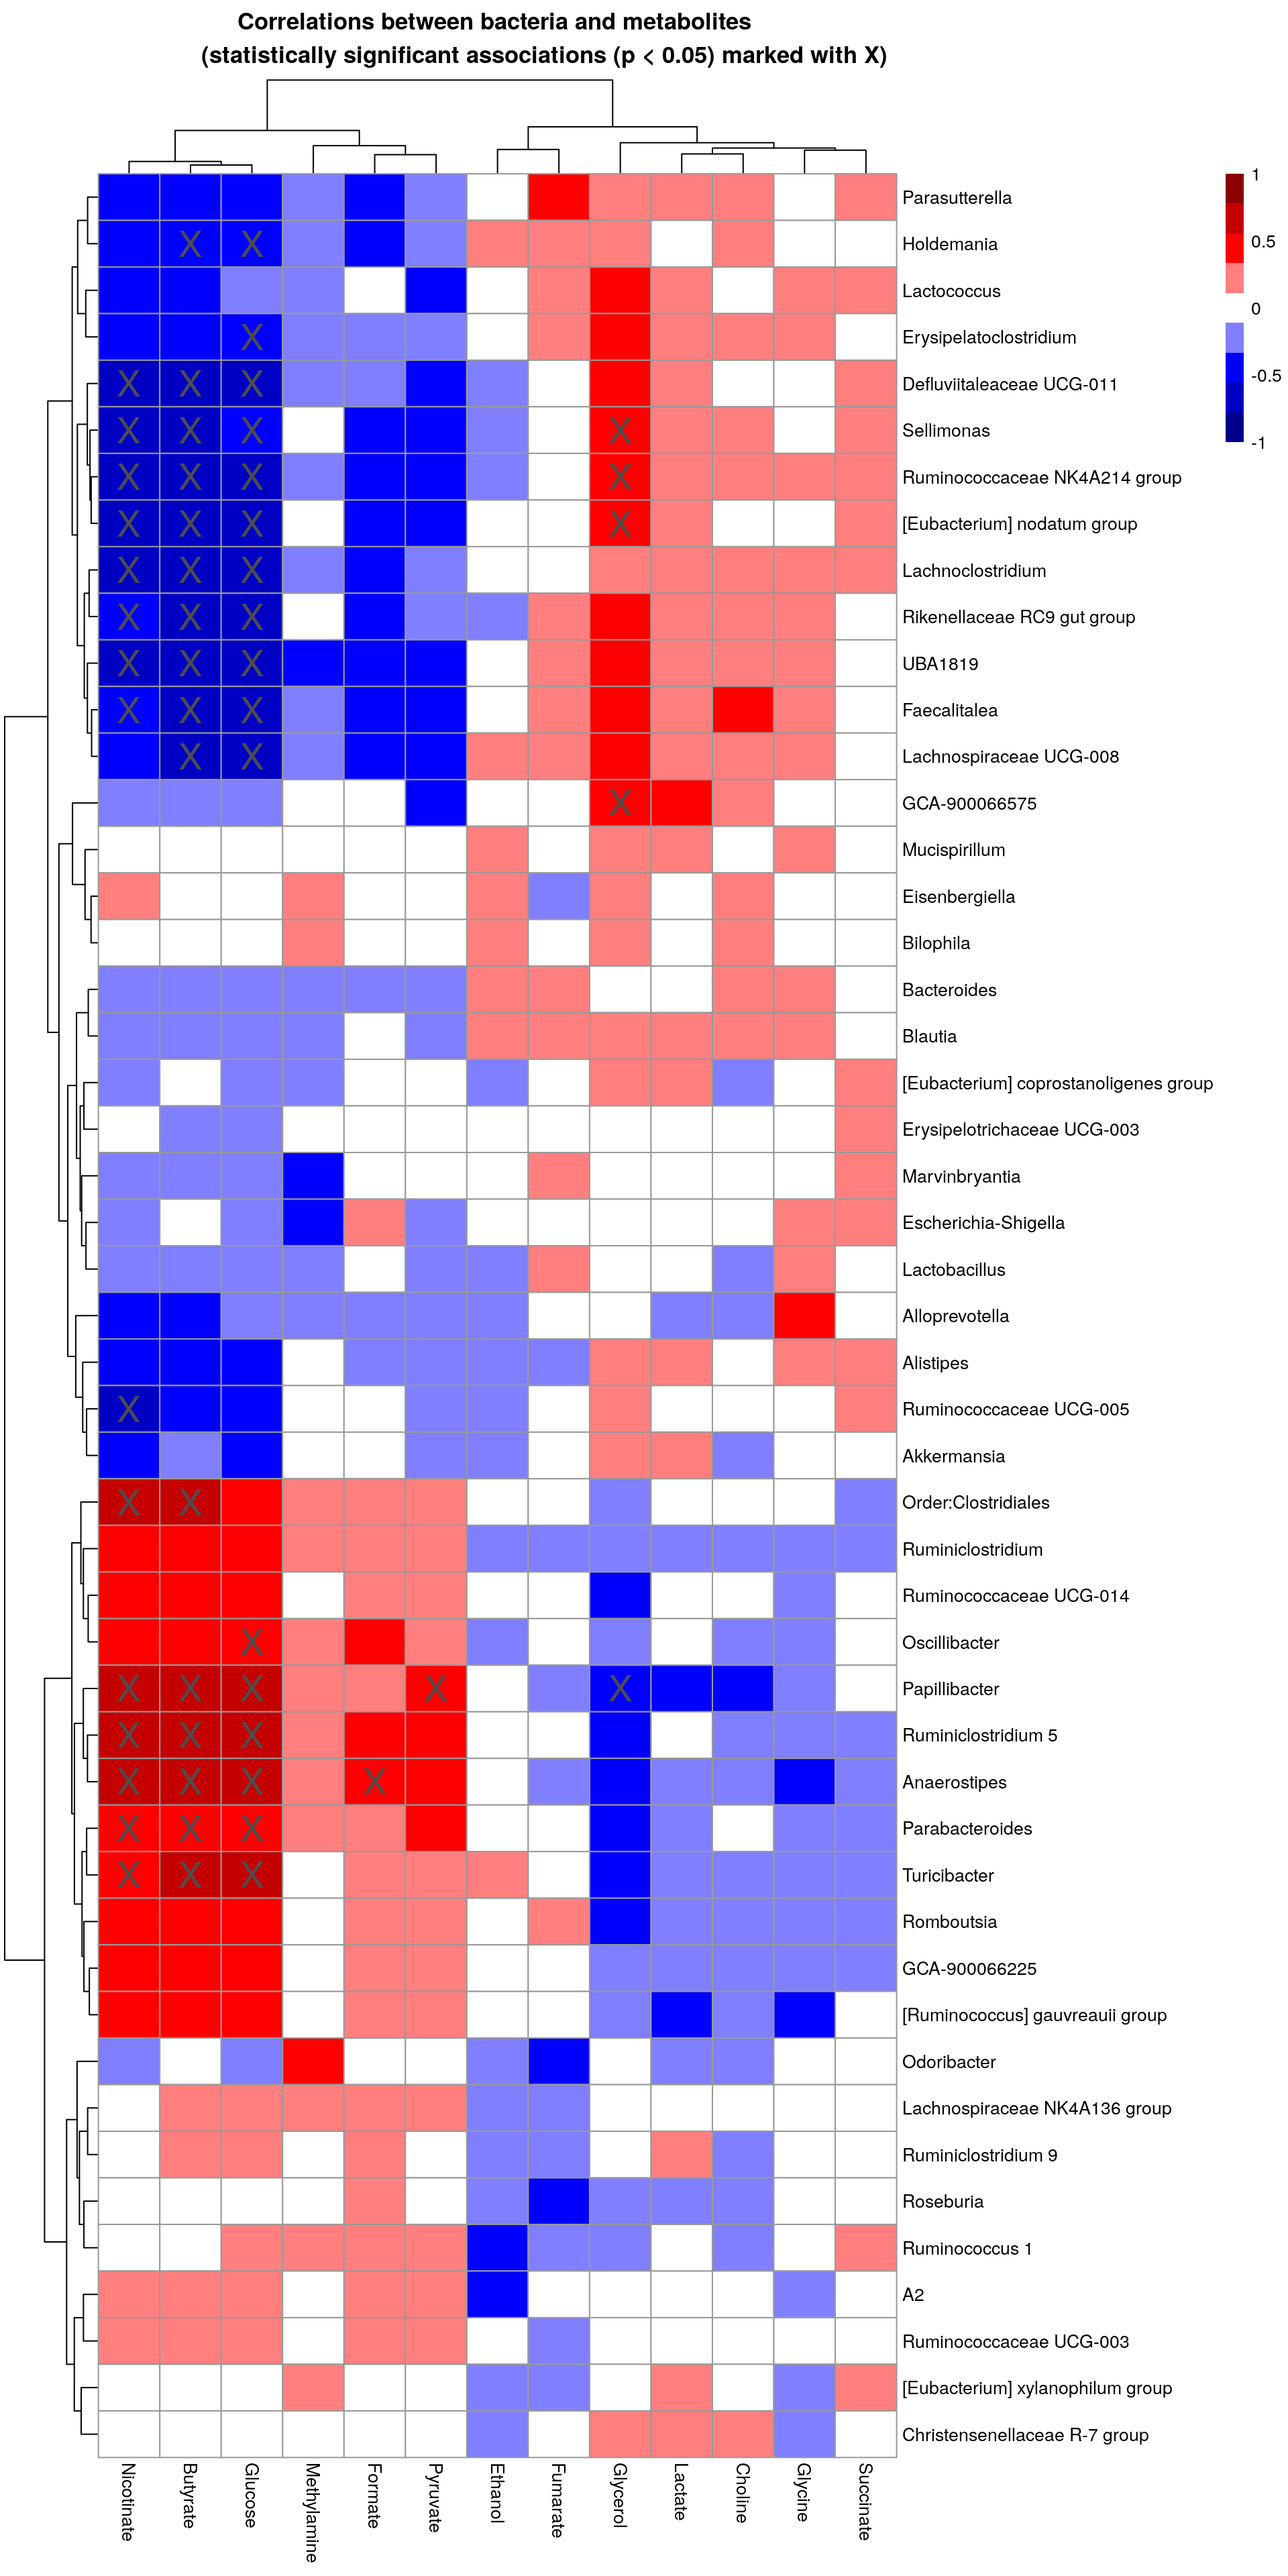
\includegraphics{06-unsupML_files/figure-latex/unnamed-chunk-5-1.pdf}

\hypertarget{supervised-learning}{%
\chapter{Supervised learning}\label{supervised-learning}}

Coming up\ldots{}

\hypertarget{model-selection-and-evaluation}{%
\chapter{Model selection and evaluation}\label{model-selection-and-evaluation}}

Coming up\ldots{}

  \bibliography{packages.bib}

\end{document}
